
%% bare_jrnl.tex
%% V1.4b
%% 2015/08/26
%% by Michael Shell
%% see http://www.michaelshell.org/
%% for current contact information.

%%*************************************************************************
%% Legal Notice:
%% This code is offered as-is without any warranty either expressed or
%% implied; without even the implied warranty of MERCHANTABILITY or
%% FITNESS FOR A PARTICULAR PURPOSE! 
%% User assumes all risk.
%% In no event shall the IEEE or any contributor to this code be liable for
%% any damages or losses, including, but not limited to, incidental,
%% consequential, or any other damages, resulting from the use or misuse
%% of any information contained here.
%%
%% All comments are the opinions of their respective authors and are not
%% necessarily endorsed by the IEEE.
%%
%% This work is distributed under the LaTeX Project Public License (LPPL)
%% ( http://www.latex-project.org/ ) version 1.3, and may be freely used,
%% distributed and modified. A copy of the LPPL, version 1.3, is included
%% in the base LaTeX documentation of all distributions of LaTeX released
%% 2003/12/01 or later.
%% Retain all contribution notices and credits.
%% ** Modified files should be clearly indicated as such, including  **
%% ** renaming them and changing author support contact information. **
%%*************************************************************************

\documentclass[10pt, onecolumn, twoside, peerreview]{IEEEtran}
\usepackage[letterpaper, margin=0.75in]{geometry}


% *** GRAPHICS RELATED PACKAGES ***
\usepackage{longtable,tabu}
\usepackage{graphicx}
\usepackage{caption}
\usepackage{pdfpages}
% declare the path(s) where your graphic files are
\graphicspath{{images/}{docs/}}
% and their extensions so you won't have to specify these with
% every instance of \includegraphics
\DeclareGraphicsExtensions{.JPG,.pdf}

% correct bad hyphenation here
\hyphenation{op-tical net-works semi-conduc-tor}

% *** CUSTOM CODE ***
% This brings in the listings package and color package so we can include code snippets into our document.
% The additional code after that is to define the Javascript language because listings doesn't have a 
% definition for Javascript.
\usepackage{listings}
\usepackage{color}
\usepackage{hyperref}
\definecolor{lightgray}{rgb}{.9,.9,.9}
\definecolor{darkgray}{rgb}{.4,.4,.4}
\definecolor{purple}{rgb}{0.65, 0.12, 0.82}
\lstdefinelanguage{JavaScript}{
  keywords={break, case, catch, continue, debugger, default, delete, do, else, false, finally, for, function, if, in, instanceof, new, null, return, switch, this, throw, true, try, typeof, var, void, while, with},
  morecomment=[l]{//},
  morecomment=[s]{/*}{*/},
  morestring=[b]',
  morestring=[b]",
  ndkeywords={class, export, boolean, throw, implements, import, this},
  keywordstyle=\color{blue}\bfseries,
  ndkeywordstyle=\color{darkgray}\bfseries,
  identifierstyle=\color{black},
  commentstyle=\color{purple}\ttfamily,
  stringstyle=\color{red}\ttfamily,
  sensitive=true
}

\lstset{
   % language=JavaScript,
   backgroundcolor=\color{lightgray},
   extendedchars=true,
   basicstyle=\footnotesize\ttfamily,
   showstringspaces=false,
   showspaces=false,
   numbers=left,
   numberstyle=\footnotesize,
   numbersep=9pt,
   tabsize=2,
   breaklines=true,
   showtabs=false,
}


\begin{document}
\title{Silicon Tracking Solutions}
%
% author names and IEEE memberships
% note positions of commas and nonbreaking spaces ( ~ ) LaTeX will not break
% a structure at a ~ so this keeps an author's name from being broken across
% two lines.
% use \thanks{} to gain access to the first footnote area
% a separate \thanks must be used for each paragraph as LaTeX2e's \thanks
% was not built to handle multiple paragraphs
%

\author{Brett~Hayes,
        Joseph~Cronise,
        and~Dylan~Camus\\% <-this % stops a space
        CS463~/~Spring~2016~/~Group 03\\% <-this % stops a space
        Final~Report
\thanks{CS463/ Spring 2016 / Group 03}% <- this % stops a space
\thanks{Final Report}}

% The paper headers
\markboth{Final Report \today}%
{Silicon Tracking Solutions}

% make the title area
\maketitle


% As a general rule, do not put math, special symbols or citations
% in the abstract or keywords.
\begin{abstract}
This document contains the work of Brett Hayes, Joseph Cronise, and Dylan Camus pertaining to the Silicon Tracking
project. This project is a web-based inventory system used by the Performance, Measurement, and Analysis team at Intel
in Chandler, AZ. The inventory system we have designed tracks the information and status of CPU silicon used by the
team and is made to help them to know where their high value inventory is at all times, as well as saving the team time
and effort towards obtaining the items they need to get their work done. We have designed for them a system such that
every time an engineer within their lab needs to use an item, they will need to check out the item through our system
and check it back in when they are done. This ensures that highly sensitive materials don't go missing without a log of
who has had ownership of the item, as well as letting others know who currently is in ownership of the item.
\end{abstract}

% For peerreview papers, this IEEEtran command inserts a page break and
% creates the second title. It will be ignored for other modes.
% \IEEEpeerreviewmaketitle
\clearpage
\tableofcontents
\clearpage

\section{Introduction} 

\subsection{Who Requested it?}
This project was requested by our client Scott, along with his team at Intel.

\subsection{Why Was It Requested?}
Scott's team needs to keep inventory of all of their CPU silicon in their lab. These silicon pieces have no real identifiable marks other than a serial number. The members of Scott's lab needed an easy way to retrieve information about the silicon. The other reason for this inventory system is to know who has which silicon. Each piece of silicon is considered very valuable to Intel, so they need a way to know who has taken silicon in order to do testing. They also want to know who has which silicon for their own team's sake. They like to know if a certain piece of silicon is being used by another team member, and to know as soon as their teammate is done with it.

\subsection{What Is Its Importance?}
It is important for the team members to have an easy-to-use system that helps them do their work more efficiently than they could without it. It is meant to save them time, and get to the important parts of their work. This system is also important in preventing the loss of silicon, which could be very costly.

\subsection{Who Was/Were Your Client(s)?}
Scott Oehrlein

\subsection{Who Are the Members of Your Team?}
Brett Hayes, Joseph Cronise, and Dylan Camus

\subsection{What Were Their Roles?}
None of the members took on a specific role for the project. There were many tasks to the project, so everyone had to take on multiple roles, with much overlap between roles. The description of the roles provided will be about which member was the primary caretaker for that part of the project.\\

Brett was responsible for the server-side implementation. He created the basic structure and maintained a lot of the server-side code. He was also responsible for a lot of the dynamic code running on the client. Brett also set-up a task list each term, to make sure the team was on track throughout the project.\\

Dylan was in charge of the database. He worked on the design structure, and created many of the stored procedures used in the current system. He was also responsible for the emailing system, which included sending immediate emails and scheduled emails.\\

Joseph came up with the original design of the website, and was responsible for the research involved in facial recognition.

\subsection{What Was the Role of the Client(s)? (I.e., Did They Supervise Only, or Did They Participate in Doing Development)}
The client played a supervisor role, and he had his team manage the setup of our project into their environment. We tried to make sure that our project was simple to set up, and would work in different environments, since we do not have any knowledge of their environment. Our client's team also took care of most of the security of the project, since that is also knowledge-based and they are the only ones with access to that knowledge.


\section{The Original Requirements Document}
This is the Requirements Document we wrote at the beginning of the
project. It has been reformatted to keep consistent styling with this document, but the content of the document has
not been modified. We have also indexed the requirements in this document for easy reference. The original document in its original formatting is included on the usb storage drive.
\subsection{Introduction}

\subsubsection{About This Document}
This is the requirements document for the Silicon Tracker project. Included in the following sections are lists of user
stories organized by categories. Each paragraph contains a feature to be added to the web application. They are all
organized into their respective categories and are set up as individual tasks to be checked off as they are
completed.\\

\subsubsection{Definitions}
The “kiosk” mentioned in a few user stories is a nickname that the Intel PMA Labs has given for their check in/check
out system. They have a computer with a QR scanner that sits on top of a large locker with all the items they store.\\

Although one of the main items being tracked will be silicon, we use the generic term “item” to specify that any part
needed, not just silicon, can be inventoried by our system.\\

\subsubsection{Current System}
The current system Intel uses is inadequate for their needs. The items have to be checked in or out one at a time. This
means the user has to enter their credentials for every item that goes through the system. They are wanting a more
user-friendly web application where they can add items to their “shopping cart” and when they are ready, go to the
kiosk and check in and out all their items in a single transaction.\\

\subsection{The Client would like to...}

\subsubsection{Inventory}
\paragraph*{Req 1} Queue an item that the user wants but is not checked in. If a person needs this item and it is currently checked out,
they can be put on a queue for that item.\\

\paragraph*{Req 2} Give a reason and a priority when queueing an item. This will create a priority queue for the users. If someone needs
an item and it is important, they can give a reason why.\\

\paragraph*{Req 3} When an item gets checked in and there were people waitlisting on the item, the people who have waitlisted will be
notified with everyone's priority and reason for needing the item.\\

\paragraph*{Req 4} Check out an item that is checked into the system. If nobody else has the item reserved, they can check out the item
immediately.\\

\paragraph*{Req 5} Check in an item that was checked out of the system. The user returns the item so other people can check out the
item.\\

\paragraph*{Req 6} Check in multiple items in a single transaction. The current system doesn't allow this feature. This would let the user
check in multiple items without giving their credentials for every item.\\

\paragraph*{Req 7} Check out multiple items in a single transaction. The current system doesn't allow this feature. This would let the
user check out multiple items without giving their credentials for every item.\\

\paragraph*{Req 8} Check in and check out multiple items in the same transaction. Along with the above two stories, the user should be
able to both check in and out and only give their credentials once.\\

\paragraph*{Req 9} Enter new items into the system. There should be a form that a user can fill out. They will scan the item to insert the
item's ID.\\

\paragraph*{Req 10} Retire old items in the system. They need to logically delete (scrap) items when an item is no longer being used. There
should be a textbox to optionally give a reason for the item being retired.\\

\paragraph*{Req 11} Be able to scan an item when checking in and have that automatically update the database. The user should just be able
to log in, and then scan the item. The status of the item should be updated based on the item being scanned. This
should happen when the user has the item currently checked out.\\

\paragraph*{Req 12} Be able to scan an item when checking out have that automatically update the database. The user should just be able to
log in, and then scan the item. The status of the item should be updated based on the item being scanned. This should
happen when the user has the item.\\

\paragraph*{Req 13} Be able to scan an item that is currently checked in to see who has the item reserved next. This will show the next
person in line for the item.\\

\paragraph*{Req 14} Be able to scan an item that is currently checked out to see who has the item checked out. For example, if there is an
item that someone left out and nobody knows who has it checked out, the item can be scanned to see who it currently
belongs to.\\

\paragraph*{Workflow of the system}

\paragraph*{Req 15} The initial screen is a welcome screen. This is where the user can scan their badge, use facial recognition, or enter a
username/password to login. After proper authorization, the user is presented with the shopping cart interface.\\

\paragraph*{Req 16} The user can now start scanning items.\\

\paragraph*{Req 17} If the item is scanned and the item is checked in, it will now be checked out by the user. If the item was already
checked out, information about who currently has the item checked out will be displayed on the screen.\\

\paragraph*{Req 18} If the current user has an item checked out, they can scan the item and the item will be checked in.\\

\paragraph*{Req 19} When the user is done, they will press a confirm button and will be shown a list of items they have checked in/out. The
user can then proceed to commit their transaction to the database.\\

\subsubsection{Security}
\paragraph*{Req 20} Log into the application with a username and password.\\

\paragraph*{Req 21} User settings and permissions will be maintained in the project database. Authenticate user credentials using the
Active Directory server already set up at Intel. They already have a system in place and the users will have to sign in
with their current credentials.\\

\paragraph*{Req 22} Authenticate facial recognition using the project database. The data stored for facial recognition will have to be in
the project database, since we cannot modify the Active Directory server.\\

\paragraph*{Req 23} When setting up facial recognition for a user, authenticate user with username and password, or with RFID tag first.
This is for security reasons, so other people won't try to scan their face on someone else's profile. When checking in
or out item(s), the user should be able to authenticate with their current RFID tags using an RFID reader.\\

\paragraph*{Req 24} When checking in or out item(s), the user should be able to authenticate with facial recognition.\\

\paragraph*{Req 25} When checking in or out item(s), the user should be able to authenticate with username and password.\\

\paragraph*{Req 26} Those with elevated permissions can retire old items from the system. This will be a logical delete, not an actual
delete from the database.\\

\paragraph*{Req 27} Those with elevated permissions can modify certain fields of the items.\\

\paragraph*{Req 28} Have any communication between the web server and the client will be encrypted through SSL. The information about the
items are all confidential, and they need to stay that way.\\

\paragraph*{Req 29} Admins will have the ability to enable/disable any of the three authentication methods (username/password, RFID tag, or
facial recognition). If for whatever reason the admin does not want one of these methods available, they can disable
that method of authentication.\\

\subsubsection{Database}
\paragraph*{Req 30} Have new items be inserted into the project database.\\

\paragraph*{Req 31} Have old items continue to be stored in the database after they are retired (logically deleted). Certain users still
need the information about items even if they are no longer active.\\

\paragraph*{Req 32}  Have a record of who checked in which items, and have that stored in the database. This creates an audit trail for all
the items.\\

\paragraph*{Req 33} Have a record of who checked out which items, and have that stored in the database. This creates an audit trail for all
the items.\\

\paragraph*{Req 34} Have a timestamp for every time an item is inserted, updated, or retired. This is also for auditing reasons.\\

\subsubsection{Services}
\paragraph*{Req 35} Have an e-mail sent out when an item is queued to any person that has the specific item checked out.\\

\paragraph*{Req 36} Send out periodic schedulable reports via e-mail to each user based on the items they checked in and out, and have on
queue.\\

\paragraph*{Req 37} Have users be notified via e-mail when they check in an item. This should happen for every transaction, so the user
doesn't get a separate e-mail for every item.\\

\paragraph*{Req 38} Have users be notified via e-mail when they check out an item. This should happen for every transaction, so the user
doesn't get a separate e-mail for every item.\\

\paragraph*{Req 39} Have users be notified when an item is now considered retired and they have the item currently checked out. They will
need the e-mail so they know to return it immediately.\\

\subsection{The Interfaces...}
\subsubsection{Main Interface}
\paragraph*{Req 40} Will be a touch interface without need of keyboard. The keyboard will still be available for certain functions, such as
entering a new item. The idea is that the user doesn't have to use the keyboard for check-in and check-out
transactions.\\

\paragraph*{Req 41} Will be able to check in items from this interface. This should not require a keyboard. The user should simply login to
the system and scan the item(s) to check them in.\\

\paragraph*{Req 42} Will be able to check out items from this interface. This should not require a keyboard. If they have the item ready
for check out, then they should simply login to the system and scan the item(s) to check them out.\\

\paragraph*{Req 43} Will be able to scan an item and display the information about that item (i.e. in the case of silicon, Core Count, LLC
Size, Frequency, Status (Checked in or Checked out), etc.)\\

\subsubsection{Shopping Cart Interface}
\paragraph*{Req 44} Will be able to check in items from this interface. If they are at the kiosk they should have a way to check in items
using this interface.\\

\paragraph*{Req 45} Will be able to check out items from this interface.\\

\paragraph*{Req 46} Will be able to add new items to the system from this interface. When a new item comes in, they will need to enter
information about the item, and then scan it so they have the serial number recorded.\\

\paragraph*{Req 47} Will be able to retire items from circulation (with elevated privileges). The items will be scrapped, but still in the
database for record keeping.\\

\paragraph*{Req 48} Will be able to reuse information of items when the same item is being added to the inventory system. They will have
multiples of the same item. That item should just be scanned and linked with the other items in the system.\\

\paragraph*{Req 49} Will be able to search for items based on certain fields in the database. The user should be able to filter their
search results based on the item attributes.\\

\paragraph*{Req 50} Will have multi-level filtering on searches. For more information, see Appendix – Multi-Level Filtering.\\

\subsubsection{Scrapping Interface}
\paragraph*{Req 51} If a user has the right elevated privileges, they can be taken to a scrapping interface. This interface will be similar
to the shopping cart interface. The difference will lie in the fact that any item the user scans will be scrapped
instead of checked in/out. They will confirm and commit their transaction, just like the shopping cart interface.\\

\subsubsection{Reporting Interface}
\paragraph*{Req 52} Will be able to view any item in circulation. This should be in the form of a user-friendly table with pagination.\\

\paragraph*{Req 53} Will be able to view any item that is retired. This should also be in the form of a user-friendly table with
pagination.\\

\paragraph*{Req 54} Will be able to see what items a certain user has checked out. They should be able to click on a user, and it will give
a list of items in a user-friendly table with pagination.\\

\paragraph*{Req 55} Will be able to search for any user who checked out a certain item. This will display as a table with the users who
have one or more of these items.\\

\paragraph*{Req 56} Will have multi-level filtering on searches. For more information, see Appendix A – Multi-Level Filtering.\\

\subsection{The Expo Should Look Like...}
\subsubsection{Web Application}
\paragraph*{Req 57} A Fully functioning version will be running during the event. This will be a system that the general audience can view
and play with.\\

\paragraph*{Req 58} Anybody can have their faces entered into the database. This will show how the facial recognition works.\\

\paragraph*{Req 59} Anybody can scan sample RFID cards to check in or out items. We will have sample items for them to scan, and they can
use fake RFID badges to simulate the experience.\\

\paragraph*{Req 60} Anybody can scroll through the different interfaces. They will have admin privileges so they can see all the features
of the application.\\

\paragraph*{Req 61} Anybody can check in or out items into the system. There will be a set of sample items people can scan so they can see
how the system works.\\

\subsection{Appendix}
\subsubsection{Multi-Level Filtering}
This is a filtering process for items that are in the database system. It is used for easy search filtering based on
multiple fields. For example, if the user is filtering items based on clock speed and they want to narrow their search
further, then they can select another field to filter on. If they decide to filter again on cache size, then they will
only see the possible filters for cache size based on the items with the specific clock speed they chose earlier.\\

\subsubsection{Gantt Chart}
\begin{figure}[H]
	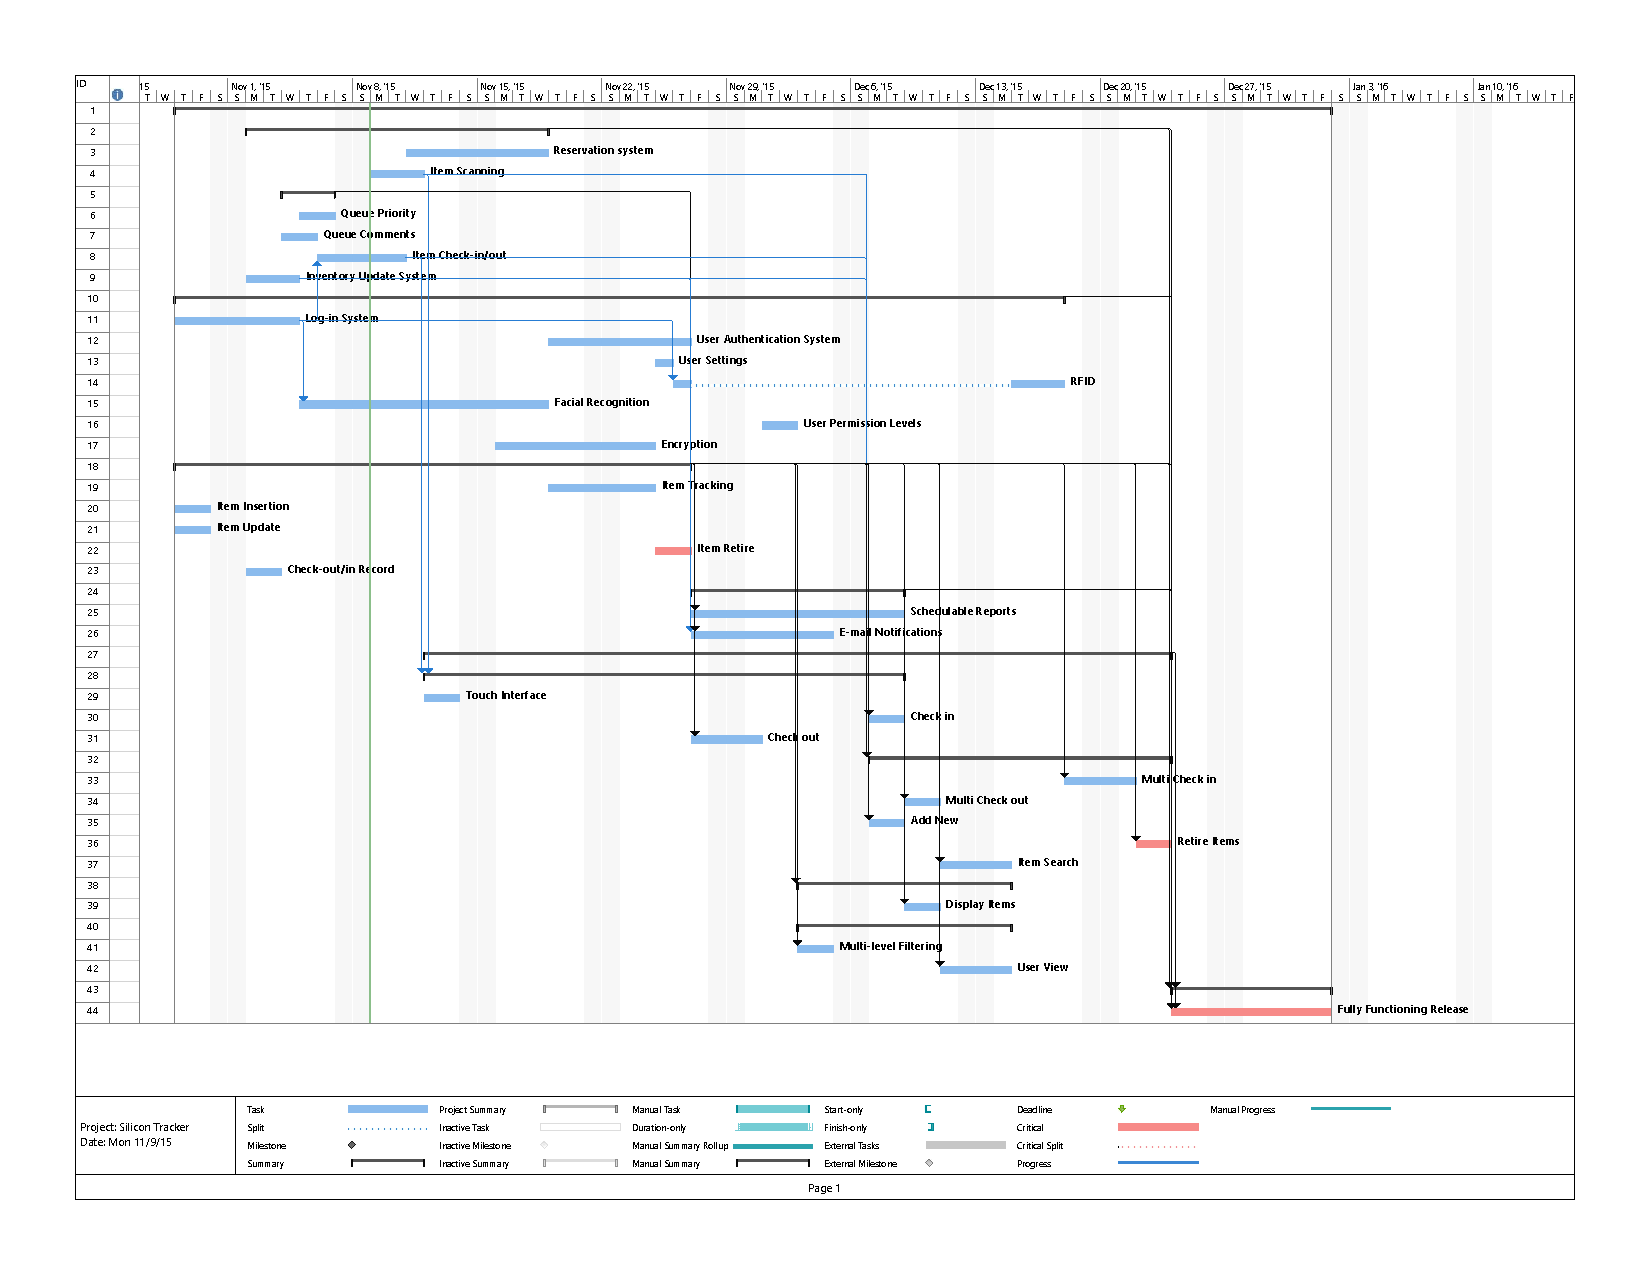
\includegraphics[angle=90, width=\textwidth]{gantt}
\end{figure}
\clearpage

\section{Changes Since the Original Client Requirements Document}

\begin{center}
		\begin{longtabu} to \textwidth {|X[1,l]|X[10,c]|X[10,c]|X[10,c]|}
			\hline
			\# & Requirement & Reason For Changes & Comments \\ \hline
			2 & Give a reason and a priority when queueing an item. This will create a priority queue for the users. If someone needs an item and it is important, they can give a reason why. & Our client stated that since they are a small team, they only needed an email stating that the item has been checked in. All the people can meet up and talk about who gets the item next. & \\ \hline
			10 & Retire old items in the system. They need to logically delete (scrap) items when an item is no longer being used. There should be a textbox to optionally give a reason for the item being retired. & There is no textbox to give a reason for the item being scrapped. Each item has a notes field, and we decided that the best option was to place the reason for scrapping in the item's notes field. & \\ \hline
			13 & Be able to scan an item that is currently checked in to see who has the item reserved next. This will show the next person in line for the item. & We decided not to be concerned about this, because everyone who reserved an item will discuss in person who needs the item next. & \\ \hline
			17 & If the item is scanned and the item is checked in, it will now be checked out by the user. If the item was already checked out, information about who currently has the item checked out will be displayed on the screen. & Our client asked if we could make it so one person can check in another's item. & \\ \hline
			19 & When the user is done, they will press a confirm button and will be shown a list of items they have checked in/out. The user can then proceed to commit their transaction to the database. & We made it so they only need to press one button to commit their transaction. A message appears now to just show what items they checked in/out, after they have committed. & \\ \hline
			29 & Admins will have the ability to enable/disable any of the three authentication methods (username/password, RFID tag, or facial recognition). If for whatever reason the admin does not want one of these methods available, they can disable that method of authentication. & Our client's team implemented RFID security, and the facial recognition was implemented very late in the development phase of the project, so we didn't get a chance to implement this setting. & \\ \hline
			N/A & The Interfaces & In our original Requirements Document, we had four interfaces. After starting work on this project, we simplified the system down to two interfaces. It made the system easier to discuss and navigate. We boiled down the interfaces into the Web interface and the Kiosk interface. The Shopping Cart interface, Scrapping interface, and Reporting interface have mostly been combined into the Web interface. The Main Interface has mostly been reworked into the Kiosk interface. & All of the requirements within the Interfaces section have been fulfilled, but not necessarily in all of the interfaces specified. \\ \hline
			44 \& 45 & Will be able to check in items from this interface. If they are at the kiosk they should have a way to check in items using this interface. Will be able to check out items from this interface. & Our client let us know that they only need to check in and check out items from one interface. Our original Requirements Document had checking in and out of items from two interfaces. We removed the Checking in and out requirements to allow for these features to happen in only one place. & \\ \hline
			59 & Anybody can scan sample RFID cards to check in or out items. We will have sample items for them to scan, and they can use fake RFID badges to simulate the experience. & Our client's team implemented the RFID readers, so we did not show how they worked at expo. & \\ \hline
			N/A & New Requirement: Sanitizing and Validation User Input & We did not place in our original document to clean up any user input and make sure that their input is valid. It was an important feature, and our client did ask that we created a system where data entered would be consistent. & \\ \hline
			N/A & New Requirement: Editing Dropdown Menu Items & We setup a page for the admins to change the dropdown menu items. These dropdowns are found when inserting or editing an item. Our client liked the idea of not having to make edits directly in the database, so we implemented this feature. & \\ \hline
			N/A & New Requirement: Quick Check in/out. & We added an extra feature for when a user scans an item to get the item's information, they can click a Check In/Out button to save the item for later. It makes it easier for the user to check in or out an item as soon as they scan it, and makes the workflow a little smoother. & Our client's team received this feature very well and were thankful to have it. \\ \hline
		\end{longtabu}
\end{center}

\subsubsection{The New Gantt Chart}
\begin{figure}[H]
  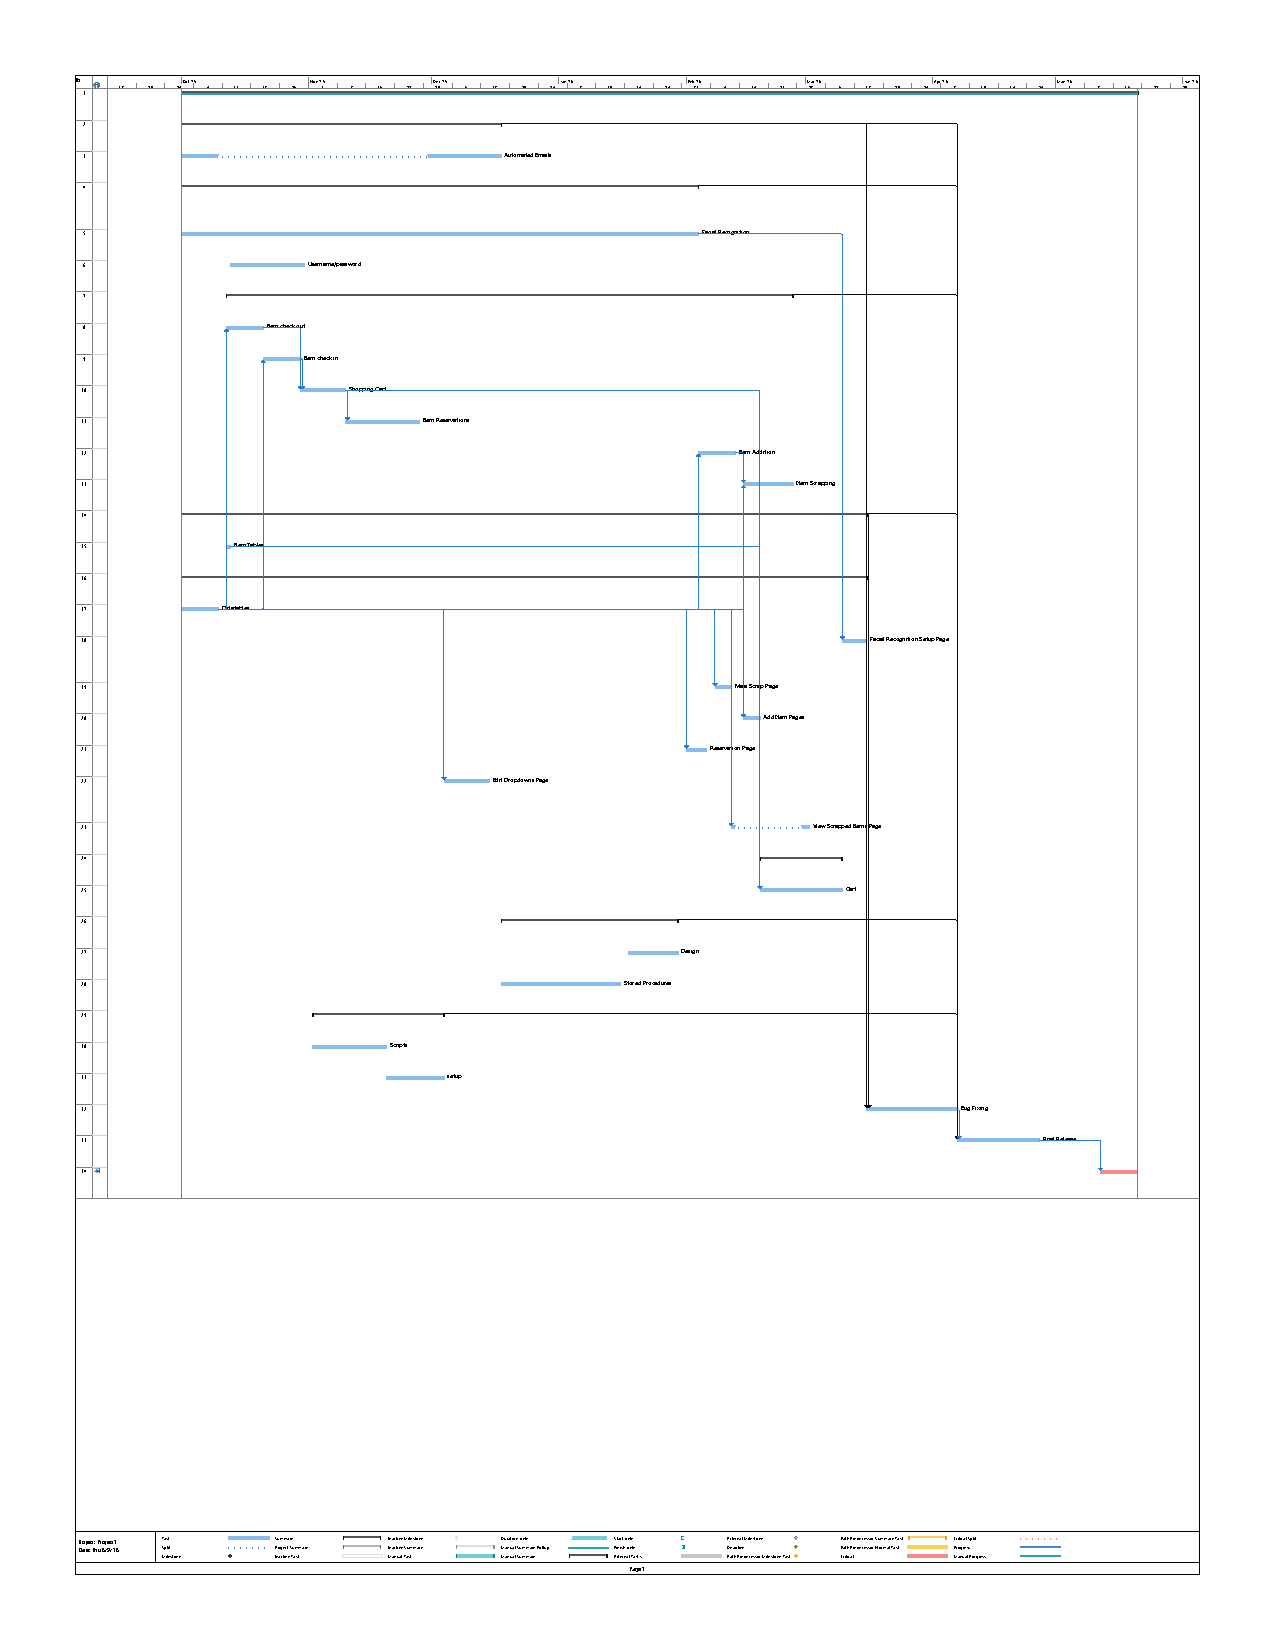
\includegraphics[width=\textwidth]{newgantt}
\end{figure}
\clearpage

\section{The Original Design Document}

Below is the original Design Document written at the beginning of the project's lifespan, in its original formatting.
It describes our course of action for designing the components, database design, and the workflow of the system. The
original document is also included on our USB storage drive.

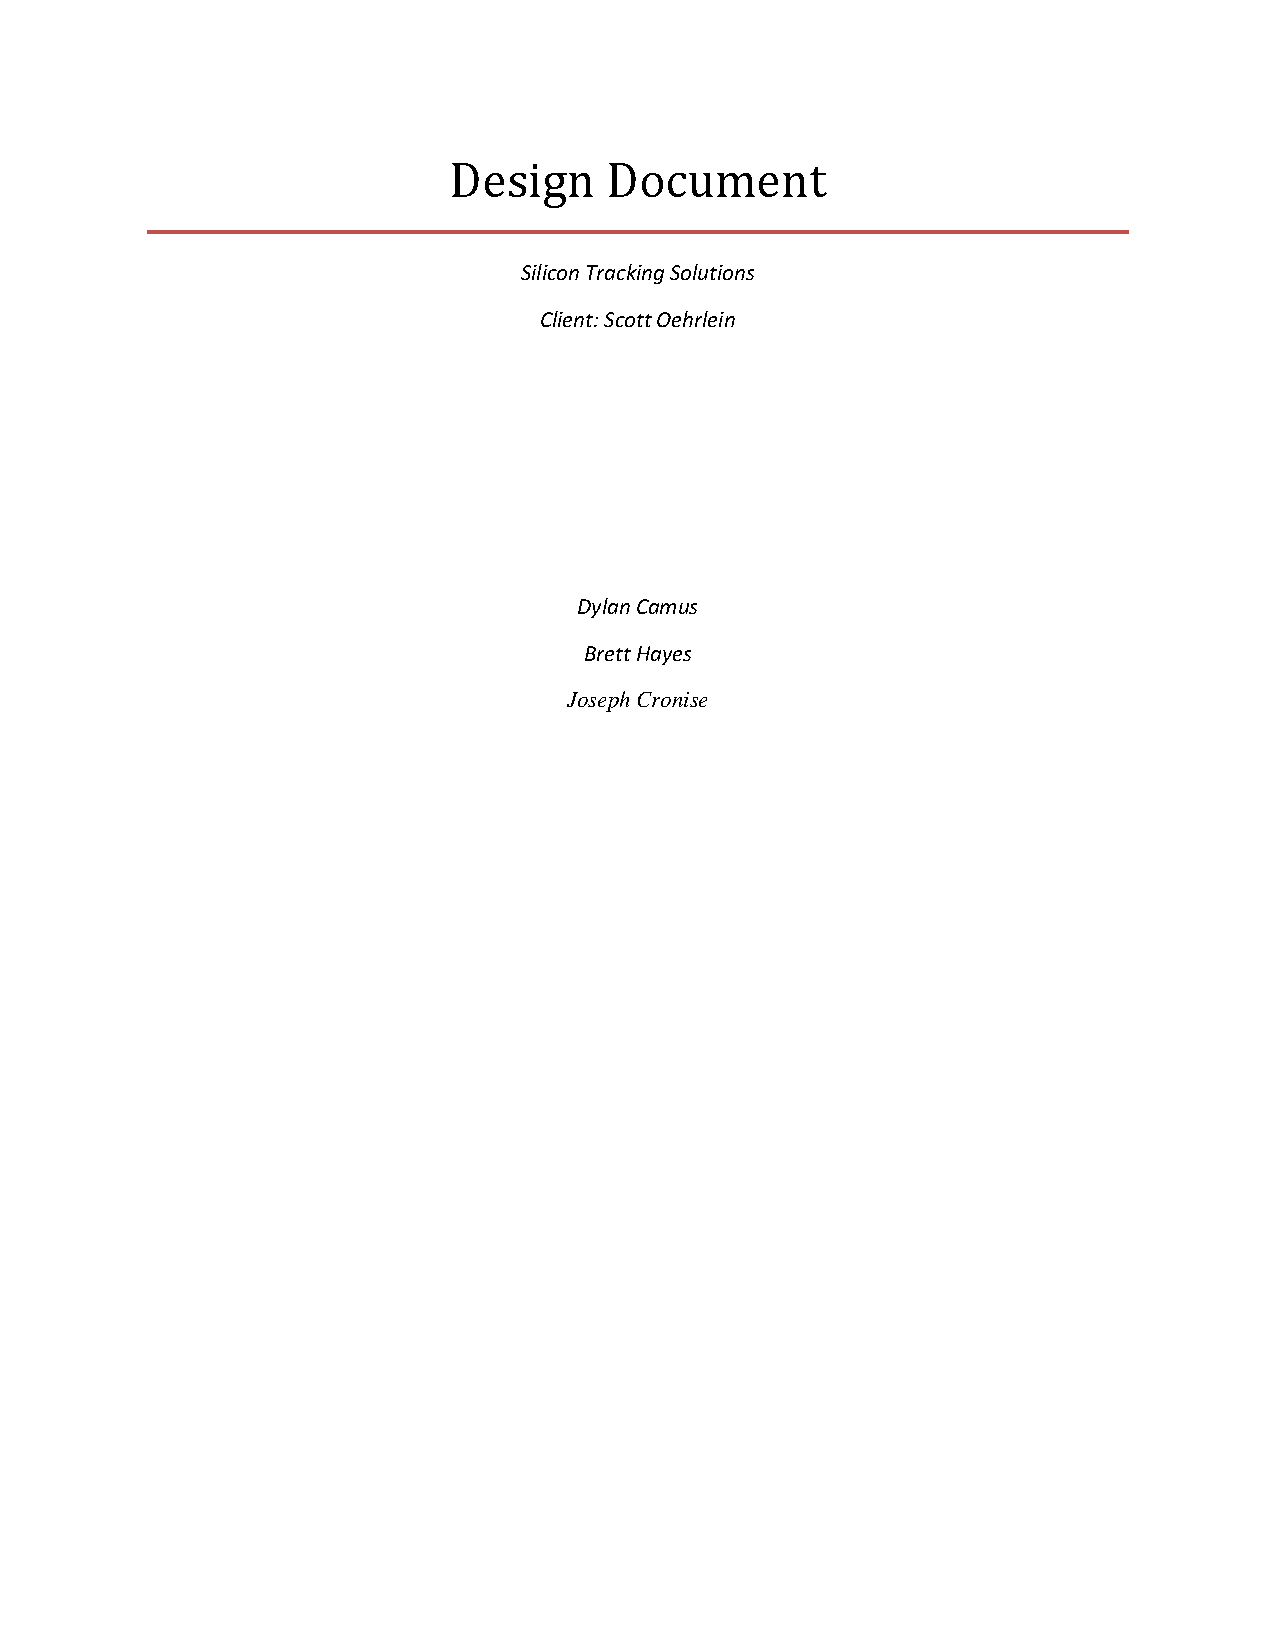
\includepdf[pages={-}]{CS461_Group03_Design_Document}

\section {Changes Since the Original Design Document}
We have changed the design of the high-level architecture. When we first started designing the project, we weren't sure on how the scanner would work. We had thought that we would have to design a separate component for the scanner to handle events and sent barcode information to the server. After playing with the scanner, we learned of its behavior and was able to handle the barcode scan as an event inside the Interface component. The scanner simulates a keyboard and presses a key for each character of the barcode it just scanned. We were able to systematically determine when a barcode was scanned and when a human was typing on the keyboard, thus having no need to separate the scanner into its own component.\\

Along with the scanner being a part of the Interface component, we also moved the Authentication component into the Interface component. We basically created only a single component that the user can have direct access to. This created a much simpler design and made it easier to develop, since there were less components all needing to communicate with the server.\\

We had originally thought we would need to create a system that authenticates users based off  an Active Directory server. After creating this document, we found out that the system would need to just send a web request to authenticate. We weren't told any more information, since that would be a security breach. We ended up creating a mock authentication system and we let our client's team handle the security from there.\\

In the Interface component, we had split the design work into two subcomponents. These subcomponents are the the Web interface and the Kiosk interface. The Web interface is for monitoring and viewing large sets of information, adding, editing, or removing items, etc. It is designed to be used for any work that would be easier to use a computer with keyboard and mouse. The Kiosk interface is designed in a way to be touch friendly, and to handle quick transactions, such as the checking in and out of the silicon chips.\\

The database schema has changed since the original design. We originally had a table for each type of item. Today we still have those item type tables, but we have a more generic table that specifies what the item type is, and references data in the more specific tables. The generic table, “Items”, holds the barcode, the notes for the item, if the item is checked in, and if the item has been scrapped, or logically deleted.\\

After a large amount of research and help from mentors, we had discovered that the SDK for the Intel RealSense Camera was not compatible with facial recognition on a web browser. This meant that we couldn't use the facial recognition software that was designed for this camera. We had to instead take two images using the RealSense camera. The camera takes an RGB image and a depth image, and uses Open Source Biometric Recognition (OpenBR), a runtime library for image processing, to do facial recognition on the RGB photo and an image comparison for the depth image.\\

\section{The Original Technology Document}
This is the Technology Document we wrote at the beginning of the project. It has been reformatted to match the styling
of this document, but the content of the document has not been modified. The original document in its original
formatting is included on the usb storage drive.

\subsection{What We Are Trying to Accomplish}
The PMA team at Intel is in need of a new inventory tracking system for their silicon and other items they need to
store. They would like a web-based inventory system where engineers can check in and check out items. All the items
tracked will need to be stored on a database. This database will need to track items and user settings. The application
will also need to communicate with the Active Directory server at Intel for user verification. Every inventory item has
a QR code that needs to be scanned when it is checked in or out. When an item is scanned, the inventory system will
update the database accordingly.

\subsection{Cameras}
\subsubsection{Standard CCTV camera}
The first possible option for the facial recognition camera would be to use a standard CCTV camera, this has the
benefit of offering a wide range of products at varying price points, as well as allowing usage of a large number of
pre-existing facial recognition software's. However, many of those software's are costly, and are more limited than an
algorithm based around the capabilities of the next two options. A CCTV camera on its own has limited functionality.
\paragraph{Cost} Varies\\

\subsubsection{Intel RealSense Camera(F200)}
The RealSense camera is Intel's 3d camera designed for laptop and tablet integration. This Camera was designed to allow
for gesture control, facial analysis, sound processing, and augmented reality. In terms of facial recognition, it has a
range of 25-75cm. The camera has three display modes, Depth, IR, and RGB. The standalone developer version requires USB
3.0, but the final product would make use of an integrated camera. It supports windows 8.1 and newer and requires a 4th
generation (or later) Intel Core processor. This camera has depth precision fine enough to detect gender, emotion, and
even the users pulse. The main drawback is the products relative newness, meaning its developer community is much
smaller as compared to the other options.
\paragraph{Cost} standalone dev kit: \$99.00\\

\subsubsection{Kinect Sensor}
The Kinect Sensor is another possible option for the facial recognition camera. This sensor, originally designed for
Microsoft's Xbox 360 and significantly improved upon with the release of the Xbox One provides much the same
functionality as the RealSense camera. It is a depth sensing camera capable of multiple modes, Color and IR, with a
stated range of 5 meters. It was designed with full motion body tracking in mind, though it is fully capable of
performing facial recognition. At 50cm the quality would be ~.75 mm per pixel. Historically the Kinect Sensor has had
issues recognizing individuals with dark skin, though Microsoft has blamed those results on lighting levels. The sensor
is also designed with the Xbox as its primary usage, there was a dedicated windows version, but that was discontinued
in favor of a simple adapter for the Xbox version. The Camera is USB powered and has a robust developer community.
\paragraph{Cost} \$99.99 + \$49.99 adapter\\

\subsubsection{Selection Criteria}
The chosen camera must be able to output an image with enough detail to successfully recognize an individual. The
output must be clear enough to differentiate between an image of a person and the actual person, and the Camera needs
to be able to integrate with current systems already in place. Due to project criteria, and the specific request of the
sponsor, the camera selected was the Intel RealSense Camera.

\subsection{RFID Reader}

\subsubsection{1126 Desktop UHF RFID Reader}
This product is USB powered and offers both read and write capability for RFIC cards. It is specifically designed for
PoS, document tracking, and access control applications and has an extensive SDK. It has the benefit of providing both
audio and visual confirmation of a successful read and its built in antenna has a range of up to 1.5 meters,
tag/environment dependent. It is designed as a desktop device and as such has no built in mounting bracket or the
ability to add one. It works with Windows, Mac, and Linux and is a sturdy, drop resistant design.\\

\subsubsection{ID CPR02.10-AD/-B RFID Card Reader}
This is a wall mounted reader which requires an external power supply. It is unable to write cards and has two possible
communications links. Serial (RS232 or RS485) or Data/Clock (Wiegand). It has a max read distance of 7cm and includes
both visual and audio confirmation of a successful or unsuccessful read. It includes both the reader, and the wall-
mounted housing. It functions with Windows, Mac, and Linux.\\


\subsubsection{pcProx82 Series}
This is a USB powered device which works with nearly all proximity, contactless, and magnetic stripe card technologies.
It is designed to add additional functionality to already existing employee ID badges by integrating them into
applications beyond simple door access. The main benefits of this technology are its versatility, ease of use, and the
fact that it has no license restrictions. It is compatable with recent windows operating systems and is capable of
sending data as serial ASCII or non-keystroke formats with an average maximum read range of 2.5-7.6cm. It includes a
Tri-state LED and beeper for read confirmation and comes with a 1 year material/workmanship defect warranty.\\

\subsubsection{Selection Criteria}
The reader must be able to successfully read all relevant data from a standard Intel ID badge as well as integrate
properly with a tablet PC. Due to project criteria, and the specific request of the sponsor, the RFID reader selected
was the pcProx®82 Series RFID reader.

\subsection{Database Management System}
\subsubsection{MySQL}
This is an open source relational Database Management System (DBM). It is one of the most widely known client-server
DBM. One of the main benefits of MySQL is that it is already integrated into existing open source softwares such as
WordPress and Drupal due to it being a part of the Linux Apache MySQL PHP (LAMP) package. Additionally, MySQL is
supported on nearly every operating system and supports many programming languages. MySQL is known to be easy to setup
and use and is the industry standard DBM. However, MySQL is known to have stability issues and suffers from poor
performance scaling.\\

\subsubsection{Microsoft SQL Server Express}
This product is the free version of Microsoft's SQL Server. The express version is open to distribute and use, similar
to open source software. It implements many of the same features as MySQL but with a better query optimizer, the T-SQL
procedural language, and a window-based management tool. However, due to being the express version, the DBM has some
limitations. For example, there is a maximum size of 10 GB per database. Additionally, there are artificial hardware
usage limits such as only one physical CPU and 1 GB of RAM can be used. Finally, SQL Server Express is limited to
running only on Windows and supports only .Net, Java, PHP, Python, Ruby, and Visual Basic.\\

\subsubsection{Oracle Database Express}
Oracle is an object-relational database management system, meaning that it supports objects, classes, and inheritance
directly in the query language. It is an express version and, like SQL Server Express, it has limitations set on data,
allowing only 4 GB. Oracle Database is generally targeted at large enterprise applications for huge corporations. It is
supported more operating systems and supports more languages than either MySQL or SQL Server.\\

\subsubsection{Selection Criteria}
Due to the nature of the project, licensing is very important. Therefore, MySQL is the clear answer due to it being
open source. Additionally, since MySQL is inherently free, it does not have any artificial limitations imposed on it
like the other options have. Microsoft SQL server and Oracle Database both lend themselves to large enterprise
applications, whereas MySQL is generally used for smaller web applications. Finally, the team has much more experience
with MySQL than the other two languages.

\subsection{Web Application}
\subsubsection{Node.js / Angular.js}
Node.js is a javascript runtime engine that runs on Google's V8 engine. We could use this as our web server. Node.js
would handle any server-side functionality, and Angular.js would handle the client-side interface. Some of the
advantages are that the system would be very scalable, testable, and reliable. Both Node and Angular are built for
event-driven, non-blocking systems. This is particularly useful since we will have a number of I/O devices working with
our application. It would also be able to run securely with SSL. There are a few downsides to these technologies as
well. There is a learning curve that would be particularly larger since we would be learning two technologies at the
same time.\\

\subsubsection{Visual Studio Community} This is a free version of Visual Studio that we could use to create the web
application. VS Community is a full IDE with everything we would need to create a fully interactive web environment.
Building an ASP.NET application would be a good option because it is such a powerful framework. The back-end would be
written in C\#, which is designed in a way to easily interact with databases, lists, string manipulation, and much
more. It comes with Linq, which allows developers to create database queries, and sort through lists seamlessly. This
is also a very large framework, and the learning curve is probably greater than any other option listed. There are also
limitations to the licensing with the free version, so that also has to be kept in consideration.\\

\subsubsection{Vanilla HTML/CSS/Javascript with PHP}
A third option would be to go without a web framework, and use a more basic approach to developing the software. We
would just write base web interfaces with HTML, CSS, and Javascript, and then use the server-side tool PHP, which is a
more minimal scripting language. This would benefit us by giving us the freedom to come up with whatever design
structure we want to use. We could essentially write the code in anyway that we feel would be best for the system
without being imposed by framework rules and guidelines. On the other side of that argument is that we could have too
much freedom and create a complex and chaotic system that is nearly impossible to understand, since we didn't impose
any coding standards. It would have a smaller learning curve at the beginning, but as the system grows it might not be
the best option.\\

\subsubsection{Selection Criteria}
As stated in other sections, licensing is very important. All three of these systems are free, but Visual Studio
Community will have some limitations that would deter us from using it. We also have to make sure that we can read
information from I/O devices, such as the RFID reader and the camera. Node.js has the ability to work with I/O systems
easily. It has the ability to run C and C++ libraries within the system, which is useful for the RFID readers and
cameras. Angular.js easily integrates with Node.js and can create dynamic web pages.

\section{Changes Since the Original Technology Document}
Because of a large learning curve for software that wasn't necessary for development, we decided not to use Angular.js, a javascript web framework, for the interface. Instead, we used only HTML, CSS, and JavaScript/JQuery for our interface, without a framework.\\

We had discovered that the SDK for the Intel RealSense Camera could not do facial recognition if the camera is being used through a web browser. Because of this, we switched to using Open Source Biometric Recognition (OpenBR), a runtime library for image processing.\\

\section{Weekly Blog Posts}
Throughout the course of the project, we wrote a weekly update on a blog post whenever there was work done on the project. Each blog post is in chronological order and styled in a way that makes it easy to differentiate between them.

\subsection{Welcome to my blog! by Cronise, Joseph Eric}
This is where I'll be sharing my thoughts on topics that matter to me. Who knows... I might even share pictures, videos and links to other interesting stuff.\\

If I catch your interest, let me hear from you.

\subsection{Weekly Update 10/23/2015 by Cronise, Joseph Eric}
​This week we held our weekly meeting with Scott Oehrlein on monday. We went over his changes to the design document as well as clarified a few matters and asked any questions we needed.\\

On tuesday we were given two Realsense cameras which were distributed to Dylan and Brett, Joseph has his own, albiet an older model. Each member took some time to briefly familiarize themselves with the camera.\\

Over the entire week we, individually, have been looking into different web framework options for the project as well as refamiliarizing ourselves in database operations.

\subsection{Weekly Update 10/30/2015 by Camus, Dylan Michael}
Again this week we held our weekly meeting with Scott Oehrlein on monday. We didn't have too much to talk about but we discussed the requirements document and planned to meet with Scott in person on Wednesday November 4th.​\\

We have continued looking at web frameworks and database options and are starting to get a much better handle on what the project will look like.

\subsection{Weekly Update 11/6/2015 by Camus, Dylan Michael}
​This week our weekly conference call with Scott was canceled because our client Scott Oehrlein was in Corvallis and we were able to meet with him in person. We went over the old web app that the Intel team currently uses and where he wanted to see improvements. We also received three RFID scanners from Scott to work with.\\

​In addition, we had our first meeting with the TA this week. We went over our requirements document and where it needed improvement.

\subsection{Weekly Update 11/13/2015 by Camus, Dylan Michael}
We had a little trouble this week due to daylight savings time. We ended up missing our weekly meeting with Scott because Arizona does not recognize daylight savings time. Additionally, because of veterans day school was canceled, and therefore we did not meet with our TA either.\\

What we did, however, was complete our revisions on the requirements document and finished the tech review. We are looking to begin working on​ our design document soon.

\subsection{Weekly Update 11/27/2015 by Hayes, Brett}
This week has consisted of a number of different tasks.\\

We talked with Scott about a week ago about adding/deleting a few user stories from the requirements document. We have bounced ideas back and forth with our client and his needs for the system. We have a new revision of the document and hopefully we this version has everyone happy.\\

We still haven't had success with the RFID cards and readers. The cards from our client are blank, and we are finding it difficult to find anyone with an RFID writer so we can put fake data on the cards. We tried the RFID readers with our student IDs but have not had any success with them.\\

We prepared our elevator speech and are ready for our turn next week to give the speech. Brett is giving the intro, Dylan is giving the problem and Joseph will deliver the solution.\\

We plan on working on the design document this weekend and will work hard on it in the beginning of next week.

\subsection{Weekly Update 12/5/2015 by Hayes, Brett}
We had a lists of concerns for this project. We placed our list of concerns into the design document and wrote about how we plan to address those concerns.\\

Brett mapped out the high-level design and how data is going to flow throughout the system in a brief but informative way. He also went into detail about how the server will be constructed and some design features we will be implementing.​\\

Joseph came up with some prototype designs for the interface. He was able to create a model of the system and what it will look like. Some screenshots of the mock-up are in the design document. Joseph also created a mapping diagram of the database.\\

Dylan wrote an interface for the Active Directory API and how we will be working with the RFID reader, facial recognition, and username/password authentication. He also wrote how the barcode scanner will be used and implemented into our system.\\

We spent most of the week on the design document. Aside from the document, we received the barcode scanner from Scott and were able to test out the scanner on some ​fake CPU silicon chips that Scott also provided.

\subsection{Weekly Update 1/16 by Hayes, Brett}
​The previous week was geared towards setting up our coding environments. This week we have been building the basic blocks of our product.\\

Dylan continues to work on the database scripts. He is ​writing what will be the CREATE TABLE scripts.\\

Joseph has been developing a skeleton of all the web pages for the project. The welcome screen has been placed on our webpage. It contains a simple username and password form.\\

Brett has set up the database that the group will use to develop the project. It is connected with the hosted website that he put up online. He is also looking into methods of how to detect when a barcode scanner and an RFID reader will be hooked up to the kiosk.\\

We had our weekly meeting with Scott on the 15th. We decided that next week we will be going over the design of the interface considering we get a few more pages online. Scott plans on visiting OSU in February, so we also discussed a good meeting time for when he is in town.

\subsection{Weekly Update 1/29 by Hayes, Brett}
Joseph has been working hard on the interface, and making it look aesthetically pleasing. He has been the primary person to work on the front-end coding. Joseph has also been working on figuring out what is needed for the RFID tags.\\

Dylan has continued to work on the database scripts. After writing the scripts to create the tables for the database, he has been working on the stored procedures that will be called when creating an item, looking up an item, etc.\\

​Brett has been working on the server-side code. He has been attempting to make the website secure through SSL security. Brett has also started looking into what it will take for an automated e-mailing system. He has begun the process of integrating OAuth authentication.\\

After our weekly meeting with Scott, we have decided to rewrite the styling of the website. He was also able to send us some sample data after the meeting so that we can begin testing some of the scripts we have written.

\subsection{Weekly Blog Post 2/5 by Hayes, Brett}
Joseph has continued to work on the interface design. He has made a lot of progress and is now waiting for our client Scott to review.\\

Dylan and Brett have been working together on the server-side code. They have made the server connect to the database and have the ability to pull data for display on the website. Brett has also made a table with multi-column filtering (one of the requirements).​\\

The next steps are building a check in/out system, writing the midterm report, and recording a video for the midterm. Our hope is to get a somewhat polished version of our website before Scott arrives to Oregon on 2/17.

\subsection{Weekly Update 2/12 by Camus, Dylan Michael}
Our client Scott reviewed the updated interface design that Joseph created and was overall satisfied with the design. However, he has some concerns over the usability on smaller resolutions.\\

Dylan and Brett continue to update the server code. They are working on getting the SSL working and adding functionality for adding items to the database through the application. Additionally, work is being done on the kiosk app to allow for checking items in and out.\\

We finished our midterm report and video. Moving forward, we are looking to have the core functionality of adding items and checking items in and out ready for when scott comes on the 17th.

\subsection{Weekly Blog Post 2/19 by Hayes, Brett}
Scott came to visit from Arizona to see the progress we had made on the site. We actually came up with a lot of progress in the past week.\\

We now have the kiosk inserted into our live site. If a user wants to view the kiosk, they will have to type in the navbar after the website '/kiosk'.\\

A user is now able to scan an item when in the kiosk interface. If the user is on the login screen, they can scan an item and the information about the item is returned for viewing. The same code will be used for implementing the check in/out sytstem.\\

In our meeting with Scott and his team (through Skype) we were able to show the current progress of our system. Scott and his team had some great feedback, and it was really good to hear what they had to say. We have a lot of details about their wants and needs in the system.​

\subsection{Weekly Blog Post 2/26 by Hayes, Brett}
Brett worked on server administration mostly. He moved the repository to a public repo on github. He also spent time writing the readme on the github page explaining how to deploy the app onto a local machine, or with little modification, to deploy to a server. The new repo can be found here: \\

\url{https://github.com/bretterism/silicontracker​}\\

Along with writing the directions and moving the repository, Brett was able to move the latest production environment to a home server. The reason for this was that our hosting space on OpenShift was handling a lot of the SSL security automatically, so we want to make sure that our app works specifically with SSL​ and implementing whatever we need for that.\\

We also didn't have our weekly meeting with Scott. He had to cancel, and we all had previously decided to set another time to get together anyways. We are currently figuring out what time works best for everone.​

\subsection{Weekly Blog Post 3/4 by Camus, Dylan Michael}
​This week we worked on getting the last of the features that need to be in before the beta implemented. Brett set up the website on a home server and set up ssl security. He also set up the github repository for our migrated code and is working on updating the checkin/out system with user profiles.\\

​Dylan updated the database to have a more efficient way to store which items are curretnly checked out. He also setup an email scheduler that sends emails over an interval. He is currently working on creating a SQL stored proceedure to only send emails to users who have had an item checked out for some length of time.\\

Joseph has been working on the facial recognition authentication. He currently has it so that the web app will select the users web cam and display the feed on the login page. He has looked into implementing the facial recognition algorithm and has it almost finished pending more testing.\\

Our meeting times with Scott have been rescheduled to 9:30 AM on Mondays.

\subsection{Weekly Blog Post 3/11 by Hayes, Brett}
This week we discussed a few of the features with Scott, and​ he responded with good feedback. We added a feature to add new attributes for the dropdown lists when adding a new item into the system. A dynamic table is loaded to create edit or delete these dropdown attributes whenever there is a change to be made.\\

​We also added a user settings page, which lets the users change some basic features if they desire. This is where the dropdown attributes are found.\\

Basically we have added a way for the user to login, and interact with the system as a user. We implemented sessions for user. Basically, the user's information is kept on the server and is passed to the client on a per-need basis. That way secure information, such as the user's WWID, can never reach the client, but their name and user settings can be reached.\\

This next week we plan to go through our requirements document and make sure we have all the requirements fulfulled. We will be working hard on writing the document and will get together in the next few days in order to create our video for the final presentation.

\subsection{Weekly Blog Post 4/8 by Hayes, Brett}
Starting back into the term, we have worked very hard at refactoring a lot of our code. ​At the end of the winter term, we had pushed a lot of code, so our code got pretty messy. We refactored it over spring break and started the term off with a clean code-base.\\

Part of the refactoring involved stripping the web template we were using for our web pages. The template did not look well on all screen sizes, so we stripped the template and have a responsive web site.\\

We have derived a task list that covers all the code-related tasks for this term. Our task list can be found here:\\

\url{https://docs.google.com/spreadsheets/d/1ue5x-tGK24JxzuKh7rXZGm6fWu7G3c6rAJPGCW_5Hcc/edit?usp=sharing}


Brett has been working on a few major projects since the beginning of the term. He has created the ability for users to edit rows on a table, as well as write notes for each row. Brett has also worked on writing libraries for form scrubbing and validation. When someone enters a form, the data gets cleaned up and ensured that all the values are in acceptable format.\\

Dylan has been working on the scrapping interface, so the users can logically delete items in the database.​\\

Joseph has been hard at work on the facial recognition software and should hopefully have a working system implemented within the next few weeks.​

\subsection{Weekly Blog Post 4/15 by Hayes, Brett}
This week we have continued to work on our tasks and have been making our software more​ robust with less bugs. Brett has just about finished with validation and sanitization of the input forms. He has also been working on making sure all the tables on the web interface display nicely.\\

​We have learned from our client that it may not be worth including the Intel logo in our work. This includes the poster and our project. So we are working on changing our poster and project to exclude the Intel logo. We are still allowed to use the word Intel in our work as long as it is used in the correct way.

\subsection{Weekly Blog Post 5/9 by Hayes, Brett}
We have forgotten the past few weeks to write a blog post, so this will be a larger post regarding what has been accomplished in the past few weeks.\\



​​\paragraph*{April 16-​​23}

We had a sanitizer validator for some of the tables, but not all of them. In this week we brought all of the tables currently in the system up to the same standard as the CPU table. The main reason why the other tables weren't at the same standard was because we were making constant changes to the structure of the tables, so once we came up with a solid standard for one table, we then made that standard for all tables.​ After getting all of the four tables in place, we added a fifth table for motherboards. These changes broght the tables into a finished state.\\

\paragraph*{April 24-30}

​We changed the way the system handled database connections. Instead of a single connection, we made a pool of connections so that people can make database requests concurrently. This speeds up the system by removing the bottleneck of the system. We had also began further development on the displaying of item information on the kiosk. If the user scanned an item on the kiosk login page, they would get an alert with the item's information. It was only considered a temporary solution, and it only displayed CPU information. So we made a nicer solution for displaying information, and a user can scan any type of item and get the information.​​​ Finally, when developing for the barcode scanning portion, we wrote a program that simulates a barcode scan. It's a command-line program that, when given a serial number, will behave in the same way as our barcode scanner and type in each character of the serial number at a very fast rate. This has helped significantly with development, and allows us to test our code that requires a barcode scanner without actually using the barcode scanner.\\

\paragraph*{May 1-​7}

​We added a few new pages to the website. They both pertain to scrapping, or logically deleting, of items. The first page is the scrapped items page. It looks pretty much identical to the main page with tables. The only difference between the two pages is that the main page shows active items, and the new page shows scrapped items. The other page that was added is the "mass scrap" page. This allows a user to scan all the items they wish to scrap, and then once they are done scanning, can submit and set all those items to scrapped.

\subsection{Weekly Blog Post 5/15 by Hayes, Brett}
We have been putting in a lot of effort this past week in preparation for expo. All of us have been working very hard at making sure everything is finished on our project.\\

Brett has run through a number of bugs and features. He has fixed an issue with loging in from one interface and that session carrying over​ to the other interface. There is also a "quick" check in/out option on the kiosk login page. Admins can also edit the dropdown menus in the add item pages.\\

Dylan has been working on adding reservations to the system, so if an item is already checked out, it can then be reserved by another user.\\

Joseph is about done with the facial recognition, and should be up very soon. He has been having trouble with different SDKs and is finally about to have a working solution.\\

We are almost prepared for expo. We just have to make sure that our system can run between our machines, instead of relying on the internet in Kelley, since the internet won't be very reliable​.

\subsection{Weekly Blog Post 5/27 by Hayes, Brett}
Due to expo being last Friday, we forgot to write our blog post last week. This blog post will contain the work accomplished within the past two weeks.\\

The week leading up to expo was filled with writing a lot of code and trying to make sure that everything was working before expo. We had finished a lot of tasks and bugs including the reservation of items, and facial recognition. The night before expo we had to stay on campus through most of the night in order to finish the project and make sure it was ready. One of the reasons we were up so late was to make sure that our system would work without hiccups at expo. That included making sure that our two laptops were sharing a database, and that our website could work if we turned the internet off of our laptops. The other reason we were up so late is because we were working on getting facial recognition to work, and we had to work on it until the last minute. The Intel Realsense Camera was really difficult to work with, and it took a lot of hours to make sure that it worked correctly.\\

The day of expo went very well. None of us had gotten much sleep, but we were all excited to show off our project and we all felt proud of our work. We ended up being between two projects that were both interesting to the general public. To our left was a virtual reality implementation, and to our right was an RC car controlled remotely. Despite our project not being quite as flashy, we still were able to show it off to a lot of people, including some people representing some of the local industries. Our client, Scott was in town for the expo and he seemed happy with the work that we had put into this project over the months.\\

We haven't worked much after expo. There was a lecture on Wednesday and Kevin talked about the report and presentation. We have two weeks to finish both of these, but we will try to submit them sooner. This next week will be dedicated towards working on these, and after that, we will be finished with our capstone project.

\section{Project Documentation} 

\subsection{How Does Your Project Work?} 
The project is broken into two interfaces.
These are the kiosk, which is used for the checking in and checking out of items, and the web interface, which is used
for visualizing the data. The kiosk should only be run on one machine. At Intel, they have a physical kiosk station
where they will run the kiosk interface from. The web interface can be accessed from any personal device.\\

The kiosk interface is made up of two pages. The first is the kiosk login page. This page contains the login methods
that our system supports. These are username and password combinations and facial recognition. The team at Intel has
added a third option, which is RFID authentication. The kiosk login page also provides functionality to look up
information of a particular item by scanning that items serial number. When scanning an item with the barcode scanner,
it will detect the input regardless of where the cursor is currently. The information will be displayed on the right
hand side, along with a button to save that item for checkout upon the next login. This saved for later storage is
periodically cleared every 30 seconds to prevent unwanted items from being added to the cart in the case that someone
saves an item for later but opts not to login. Finally, the last portion of the kiosk login page is the facial
recognition interface. Users who have previously setup facial recognition will see their names in the table below the
username and password fields. They can select their name and press the facial recognition button to attempt to login
through facial recognition. It is important to look directly at the camera during the facial recognition process.\\

Once the user is authenticated, they will be introduced to the cart page. This page contains two tables, one for items
to be checked in and one for items to be checked out. Items are scanned into the tables by scanning the item's barcode
with the serial number scanner. Similar to the login page, the cursor's location is not important when scanning a
barcode. After all items are scanned, simply pressing the submit button will complete the transaction.\\

The web interface, on the other hand, has many more pages. The first page a user will be greeted with upon entering the
URL is the homepage. This page contains tables which list every item currently in the database. The different tables can
be accessed by clicking on their corresponding tabs. Items can be searched in the table using a multi-column search. For
example, one can search for all 4 core CPUs that also have a frequency of 2.5. Each entry in the table also has a button
for adding notes. Clicking on the button creates a dropdown field for entering the note. If the user is logged in the
admin privileges, each entry in the table will have yet another button. This button is for editing the items fields.
Clicking on the button causes a modal to appear which contains a form filled with all of the items current values. Items
can also be scrapped, or logically deleted, from this form.\\

The next page of the web interface is the add items pages. Clicking on the add items button in the navbar brings down a
list of possible items that can be added to the database. Each add item page contains a form for adding the items. The
forms are set up to sanitize and validate the data to make sure it is consistent and correct. Attempting to add an item
incorrectly will produce an error below the field and the item will not be added to the database.\\

The next button on the navbar will bring the user to the reserve items page. This page is only accessible if the user is
logged in. The page is similar to the homepage, except the table is only populated with items that are available for
reservation. An item is only available for reservation if another user currently has that item checked out. A user may
click on a third new button in an entry of the table to reserve the item. Once the item is reserved, the button will
change to a different icon, and clicking the button again will inform the user when that item was reserved by them. Once
the reserved item has been checked back in, that user will receive an email informing them that the item is now
available for checkout.\\

The second to last button on the navbar will bring the user to the mass scrap page. This page is only accessible from
users with admin privileges. This page is used for quickly scrapping a large quantity of items. Items are scanned into
the table just like the cart page on the kiosk. Once the user has finished scanning the items he wishes to scrap, he/she
must only press the submit button to scrap each item at the same time.\\

The final page of the web interface is the view scrapped page. This page also requires admin privileges. This page is
for viewing the retired items that are no longer in use. It also is useful if an item has been scrapped by mistake,
since the item can be found this table and un-scrapped by clicking the the edit item button.

\subsection{How Does One Install the Project?}
NOTE: We developed our project on Ubuntu, and our instructions are written assuming you are at least using a Debian version of Linux.\\

Our project is running on a Node.js server. Node.js can be downloaded from their website: https://nodejs.org. There is also a bash script in the root directory of our project to easily download and install node. Look for nodeinstall.sh. The latest version of Node should be fine. It will work with the stable or bleeding-edge version of Node.js.\\

After installing Node.js, navigate to the root folder and in the terminal type npm install. This will install any dependencies our program depends on. We use npm for all our packages. It comes installed with Node.js. For more information on npm, visit their website: https://www.npmjs.com/.\\

Our server uses a MySQL database. This can be installed either through a package manager with the command “sudo apt-get install mysql-server” if your using a debian distrobution of Linux, or directly from the binary on their website: https://www.mysql.com/downloads/. We use the MySQL Community Edition.\\

Facial recognition is done using OpenBR which needs to be installed on the server prior to facial recognition working. From the server, open a terminal window and type these commands:

\begin{lstlisting}[language=bash,title={Install GCC4.9.2}]
  sudo apt-get update
  sudo apt-get install build-essential
\end{lstlisting}


\begin{lstlisting}[language=bash,title={Install CMAKE3.0.2}]
  sudo apt-get install cmake cmake-curses-gui
\end{lstlisting}

download OpenCV 2.4.11 from:\\
\url{https://sourceforge.net/projects/opencvlibrary/files/opencv-unix/2.4.11/opencv-2.4.11.zip/download}\\
After downloading, unzip opencv-2.4.11.zip
\begin{lstlisting}[language=bash,title={Download and Install OpenCV2.4.11}]
cd opencv-2.4.11
mkdir build
cd build
cmake -DCMAKE_BUILD_TYPE=Release ..
make -j4
sudo make install
cd ../..
rm -rf opencv-2.4.11*
\end{lstlisting}

\begin{lstlisting}[language=bash,title={Install QT5.4.1}]
sudo apt-get install qt5-default libqt5svg5-dev qtcreator
\end{lstlisting}

\begin{lstlisting}[language=bash,title={Get OpenBR}]
git clone https://github.com/biometrics/openbr.git
cd openbr
git checkout v1.1.0
git submodule init
git submodule update
\end{lstlisting}

\begin{lstlisting}[language=bash,title={Build OpenBR}]
mkdir build
cd build
cmake -DCMAKE_BUILD_TYPE=Release ..
make -j4 NOTE: for faster install use more threads.
sudo make install
\end{lstlisting}

At this point you need to open the Qt Creator IDE using the command 'qtcreator \&' NOTE: this requires a gui interface to be installed on the server. this is NOT a command line utility, however once OpenBR is installed the gui is no longer required. The gui we used was Ubuntu Desktop. This can be installed via package manager. In our case, this was "sudo apt-get install ubuntu-desktop".\\
From the Qt Creator "File" menu select "Open File or Project...".\\
Browse to your pre-existing build directory "openbr/build" then select "Next".\\
Select "Run CMake" then "Finish".\\
OpenBR should now be installed on the server and facial recognition should be functional.

\subsection{How Does One Run the Program?}
There are two main interfaces to the app.\\
\begin{enumerate}
  \item The web interface
  \item The kiosk interface.
\end{enumerate}
The web interface can be found at the base url. To use the kiosk interface you must navigate to the /kiosk page. For example: the kiosk interface looks like: \url{silicontracker.xyz/kiosk}\\

We also have a second app that we have created to mock the credential login system at Intel. It's a very simplified version of their credential system (It's not actually how Intel deals with security. Our code is more of a placeholder). You will need to run this app if you plan on logging in as a user. open up a separate terminal window and go to the cred/ folder. There you will see a single file cred.js. Run this app with node cred.js.\\

The node.js app uses environment variables, and they are not included on the repo (no need for the world to know my passwords). In order to make the environment variables work, you must create a new file in the root directory called env.js.
The file should look like the following, with your own settings to replace the ones here:

\lstinputlisting[language=JavaScript,title=env.js]{code/env.js}

There are three things needed to get the database up and running:\\
\begin{enumerate}
  \item Creating the database
  \item Creating a user for the database
  \item Populating the database
\end{enumerate}

All of the database scripts we use are in the dbscripts folder. In a terminal window, navigate to that folder and login to your MySql client as root or as someone with sufficient privileges:
\begin{lstlisting}[language=bash]
mysql -u root -p
\end{lstlisting}

After logging in, the first step is to create the database:

\begin{lstlisting}[language=bash]
mysql> CREATE DATABASE tracker;
\end{lstlisting}

We called the database 'tracker' but you can rename it if you like. Just remember what you decided to call it. After creating, make sure to select the right database:
\begin{lstlisting}[language=bash]
mysql> USE tracker;
\end{lstlisting}

Once the database is created, we need a user with the right privileges to be in charge of the database.
\begin{lstlisting}[language=bash]
mysql> CREATE USER 'tracker_user'@'localhost' IDENTIFIED BY 'SomePassword';
\end{lstlisting}

You can change the name of the user if you like, but just remember what you named it.
Next, we have to populate our newly-created database. The create scripts for the tables and stored procedures, as well as insert scripts for our sample data are in the script tracker.sql located in the dbscripts folder. We will be executing this script:
\begin{lstlisting}[language=bash]
mysql> \. tracker.sql;
\end{lstlisting}

We will need to add a few permissions to our new user. It needs to select, update, and insert into the tables as well as execute stored procedures. This user will never be deleting rows, so it doesn't get that privilege.

\begin{lstlisting}[language=bash]
mysql> GRANT SELECT ON tracker.* TO 'tracker_user'@'localhost';
mysql> GRANT INSERT ON tracker.* TO 'tracker_user'@'localhost';
mysql> GRANT UPDATE ON tracker.* TO 'tracker_user'@'localhost';
mysql> GRANT EXECUTE ON tracker.* TO 'tracker_user'@'localhost';
mysql> GRANT DELETE ON tracker.Checkout TO 'tracker_user'@'localhost';
mysql> FLUSH PRIVILEGES;
\end{lstlisting}

At this point, we should have our database completely set up.
After setting up the server and downloading the dependencies, you should be able to start it up with npm start. Make sure you are in the root folder for the project before you run that command. You should be greeted with a message: 'Silicon Tracker Server listening at (ip address):(port)'. In your browser, navigate to that ip address. Don't forget the port! At this point you should be greeted with the Silicon Tracker website.

\subsection{Are There Any Special Hardware, OS, or Runtime Requirements to Run Your Project?}
There are not many specific requirements for the project, however there are a few. Facial recognition requires the Intel Realsense camera as it needs both the RGB and Depth cameras to function. Since the client side portions of the project are web based they will work with most any OS with a gui interface, though due to an issue in Linux where device names are truncated, it works better in Windows. For an unknown reason the web portions of this project do not function when using the Edge internet browser, but they work correctly in Firefox and Chrome.\\

The server side code was designed with a linux server in mind, and the code would require modification to work on a Windows server. The installation instructions and facial recognition script were also designed under the assumption that the server would be running Linux. The specific facial recognition algorithm used has a different set of installation and usage instructions for Windows and will not function as is on a non Linux server. 

\section{How Did You Learn New Technology?}
\subsection{What websites were helpful? (Listed in order of helpfulness.)}
There were many helpful websites used during this project. Ranked in order of helpfulness they would be:
\begin{enumerate}
  \item Stack Overflow
  \item Github
  \item Datatables.net
  \item Intel.com
\end{enumerate}

\subsection{What, If Any, Reference Books Really Helped?}
Only one book was used during this project as the majority of our information came from online, the book was Javascript: the Good Parts by Douglas Crockford, which was, as the title suggests, used when working with JavaScript for the server.

\subsection{Were There Any People on Campus That Were Really Helpful?}
There were two people who were helpful in completing the project. Kevin McGrath and our client, Scott Oehrlein, both provided a great deal of help and suggestions for numerous parts of the project, but most of the help came when dealing with facial recognition and the Realsense SDK.

\section{What Did You Learn From This? (Dylan Camus)}
\subsection{What Technical Information Did You Learn?}
I felt like I learned an enormous amount of technical knowledge over the course of this project. Coming into the project in the Fall I had very little web development experience. The only website I had ever built was a very simple checkout system using php for my intro to databases class.\\

The first major technology I learned was Javascript. Our project was written almost entirely in Javascript, and starting out I had almost no knowledge of Javascript. I learned how to write asynchronous code using callbacks, which our application made extensive use of. I learned how to structure a client server application in a model view controller format. I learned about the REST api and how to build a dynamic web application. I learned how to use tools like JQuery and Bootstrap to increase my productivity. I learned how to use git in a real project environment with a production branch and a development branch.

\subsection{What Non-Technical Information Did You Learn?}
I learned a lot about client interaction. We spoke over the phone with our client every week to talk about how the project was coming along. We also had a conference meeting with our client's coworkers about features that they liked, didn't like, and would like to see implemented. I also learned how to edit videos.

\subsection{What Have You Learned About Project Work?}
I learned that project work really helps productivity. I found that I would work much better when the entire team got together to work on the project at the same time because I could work out any difficulties I was having with the team. I also learned that working in a group is very helpful because of the diverse skillset each member brings to the table. Both of my group members possessed skills that I myself did not and it was useful to learn from them.

\subsection{What Have You Learned About Project Management?}
I learned that proper documentation is important. I felt that the first term was helpful because it gave me a good feel for the rest of the project. I also learned that keeping in contact with the client is extremely important for project management. Our client was very helpful at identifying bugs and giving feedback on the interface design.

\subsection{What Have You Learned About Working in Teams?}
I learned the importance of communication within a group. It is important to split up the work and make sure that everyone knows their own duties. There were times two people were working on the same task and productivity was wasted. It is also important to communicate to make sure everyone is on the same page and knows the direction we are going in. I learned that it is important to get the group's opinion before moving in a different direction.

\subsection{If You Could Do It All over, What Would You Do Differently?}
I would have put a greater emphasis on the facial recognition portion of the project. We did not value the facial recognition as all that important for most of the project and considered it as a cuttable feature. However, facial recognition was a required part of the project. By putting it off, we caused ourselves a lot of unnecessary stress when we scrambled to get the facial recognition portion of the project working.


\section{What Did You Learn From This? (Brett Hayes)}
\subsection{What Technical Information Did You Learn?}
I learned a lot about system architecture and how components can be separate and interact with each other. Along with architecture, I felt like I got real experience on workflow, and making sure everything works as one cohesive entity. I learned to think about how changing one part of the system can affect other parts. This is especially true with an event-driven system, such as this one. Along with being event-driven, our system is completely asynchronous. It was a challenge learning how to think asynchronously, and to make sure everything works even if executed out of order.

\subsection{What Non-Technical Information Did You Learn?}
I learned a great deal about customer relations. We had a great client, and he was very knowledgeable in technology, so I felt we were lucky in that aspect. However as with any client, he didn't know exactly what he wanted from the project. He knew what core components he wanted to see in the system, but it took a lot of trying new things and seeing if our client liked the work we did or not. He also knew how the system was going to be used in production, so we had to rely on him for feedback in those areas. Overall, I learned much about how to effectively communicate ideas and software with a client.

\subsection{What Have You Learned About Project Work?}
There were times when the project was near completion, and I realized that we should have taken another design or chosen another piece of technology for a component in the system. I feel like it is okay to come up with these discoveries. I wouldn't have known that our choice in technology wasn't ideal until it was too late anyways. With that, I've also learned that code can be messy, and it's not always an option to go back and refactor the entire project.

\subsection{What Have You Learned About Project Management?}
I have learned that task lists and organization are key practices. Over the winter we didn't keep a strong task list and we stressed about how much work needed to be done. At the beginning of the spring, I came up with a task list for everything that needed to be done in order to push the software to production. We tracked requirements, user stories, task assignments, the status of the task, and estimated hours. It took out a lot of guessing to how much work was left to finish the project.

\subsection{What Have You Learned About Working in Teams?}
I have learned that communication is a big factor. It really helps when each member of a team communicates what task they are currently working on, and where they are on the project. This can lead to receiving help if one of the members is stuck, and making sure that two people aren't trying to accomplish the same task.

\subsection{If You Could Do It All over, What Would You Do Differently?}
There was some additional work that the client requested but wasn't in the original requirements document. If I could go back and do it all over, I would have made sure that the work in the requirements document was completed first before attempting any additional work. We ended up completing everything, so it all worked out in the end, but it did add a lot of stress and hours to the project.


\section{What Did You Learn From This? (Joseph Cronise)}
\subsection{What Technical Information Did You Learn?}
I learned a lot of technical information during the course of this project, ranging from new languages to new APIs. While, in the end, the project did not make use of the RealSense SDK, I learned a great deal about it while I was trying to make it work for our project. This also led me to learning C\# as many of the Realsense samples were implemented in C\# and the SDK had complete functionality with that language. I also expanded my understanding of javascript, previously I had only used it for websites, but during the project I had to use it to write server side scripts for the facial recognition system. I also learned how to work with bootstrap and the datatables API for the website as well as how to integrate webcams with a website.

\subsection{What Non-Technical Information Did You Learn?}
During this project I learned a lot about what I think of as real world coding. Instead of the specific instructions you get when taking a class, you are instead given a goal and, with some exceptions, it is left up to you as to how to reach that goal. Working with an actual client gave me a greater understanding of it works to create a real product that is going to be used, and it also gave me an understanding of just how easy it is for feature creep to occur.

\subsection{What Have You Learned About Project Work?}
During this project I learned a lot about project work and how it differs from the typical assignments given out in classes. I learned how easily project creep can occur, and how important it is to keep a clear set of goals from project start to finish. This project helped to give me a sense of how coding in a work environment might go and how multiple people can work together on different parts of a larger project and still work to create a cohesive project without stepping all over each others code in the process.

\subsection{What Have You Learned About Project Management?}
I wouldn't say that I learned a lot of new information about project management during this project. Coming from a business background I had already taken many of the project management courses and new a lot about what to expect going into a project of this nature. That said, I did learn just how important it is to keep a task list and keep it updated, and attempting to create the gantt chart for this paper taught me the importance of keeping clear records of who did what task, when they started, and when they finished.

\subsection{What Have You Learned About Working in Teams?}
By working as part of a team, I feel that we were able to create a product far better than anything each of us could have created individually. I learned that, by working as a team, we were able to leverage each person's individual skills and help everyone on their tasks as needed. Even something as simple as being able to bounce ideas off my teammates was incredibly helpful when it came to completing my tasks, and I would not have been able to implement the facial recognition system as well as it was without the help of my team.

\subsection{If You Could Do It All over, What Would You Do Differently?}
If I was starting over from scratch I would do a few things differently. I would have done much more research into the RealSense's capabilities earlier in the project cycle. This would have spared me a great deal of headache when it came time to make use of the SDK to write the facial recognition code, only to realise that the SDK has only partial javascript support, and no support for running its algorithms server side while the camera is client side. I would have written our kiosk in C\# and made it an executable instead of creating it as a web interface. Had I done this I would have been able to make use of most of the RealSenses SDK, however I would have still had to implement my own database for it as the two functions required to save and load the recognition database within the SDk are non functioning.

\section{Appendix 1: Essential Code Listings}
App.js is the main entry point into the server. It is responsible for the main setup of the system, and it calls other files to help with the setup.

\lstinputlisting[language=JavaScript,title=app.js]{code/app.js}

Since we implemented our system to use the REST Api, we have many routes setup for different functionalites. For example, this route gets all the CPU silicon that has not been scrapped. It returns JSON back to the client, so the client can display the information in a table.

\lstinputlisting[language=JavaScript,firstline=63,lastline=98,title=data.js]{code/data.js}

As long as there is a need to talk to the server, there is a route that handles it. Here we can see some more basic routes that handle adding and updating items.

\lstinputlisting[language=JavaScript,firstline=114,lastline=131,title=web.js]{code/web.js}
\lstinputlisting[language=JavaScript,firstline=216,lastline=235]{code/web.js}

If the user wants to login to our system, they will need to go through this route. Note that this is an authentication system that we created, and will look differently for Intel and their security system.

\lstinputlisting[language=JavaScript,firstline=514,lastline=602,title=web.js]{code/web.js}

Here is a route that handles many things, but the important thing to note is that it is called when a user submits a transaction after scanning items to be checked in or checked out.

\lstinputlisting[language=JavaScript,firstline=170,lastline=302,title=kiosk.js]{code/kiosk.js}

Here is the code that sends the list of serial numbers from the client side to be checked in or out.

\lstinputlisting[language=JavaScript,firstline=53,lastline=68,title=cart.js]{code/cart.js}

Depending on your love for JavaScript, here is some fun code that handles the facial recognition on the client.
After taking images on the client-side, the system sends those images to the server to be saved to the database.

\lstinputlisting[language=JavaScript,title=facial.js]{code/facial.js}

Some even more fun code than the facial recognition is the code that handles barcode scanners. It checks for key presses that happen very rapidly. That is how it determines if there was a barcode scan vs a human typing.

\lstinputlisting[language=JavaScript,firstline=91,lastline=137,title=cart.js]{code/cart.js}

On our main page, there are a number of tables. Here is how we implemented the CPU table. It utilizes DataTables.js, a JQuery library for creating dynamic tables. As you can see from the code below, there are a lot of events and settings involved to get the tables just the way we want them.

\lstinputlisting[language=JavaScript,firstline=23,lastline=155,title=table.js]{code/table.js}
\lstinputlisting[language=JavaScript,firstline=647,lastline=798]{code/table.js}

Below are the scubbers and validators for all the items. The scrubbers are in charge of converting the data into usable formats, and after the data has been scrubbed, it goes through the validator to make sure the input the user added was valid. If the input was not valid, the system will send the client an array of messages to let them how how to remedy the issues.

\lstinputlisting[language=JavaScript,title=scrubbers.js]{code/scrubbers.js}
\lstinputlisting[language=JavaScript,title=validators.js]{code/validators.js}

\section{Appendix 2: Additional Photos}
\begin{figure}[!ht]
    \centering
    \captionsetup{justification=centering}
    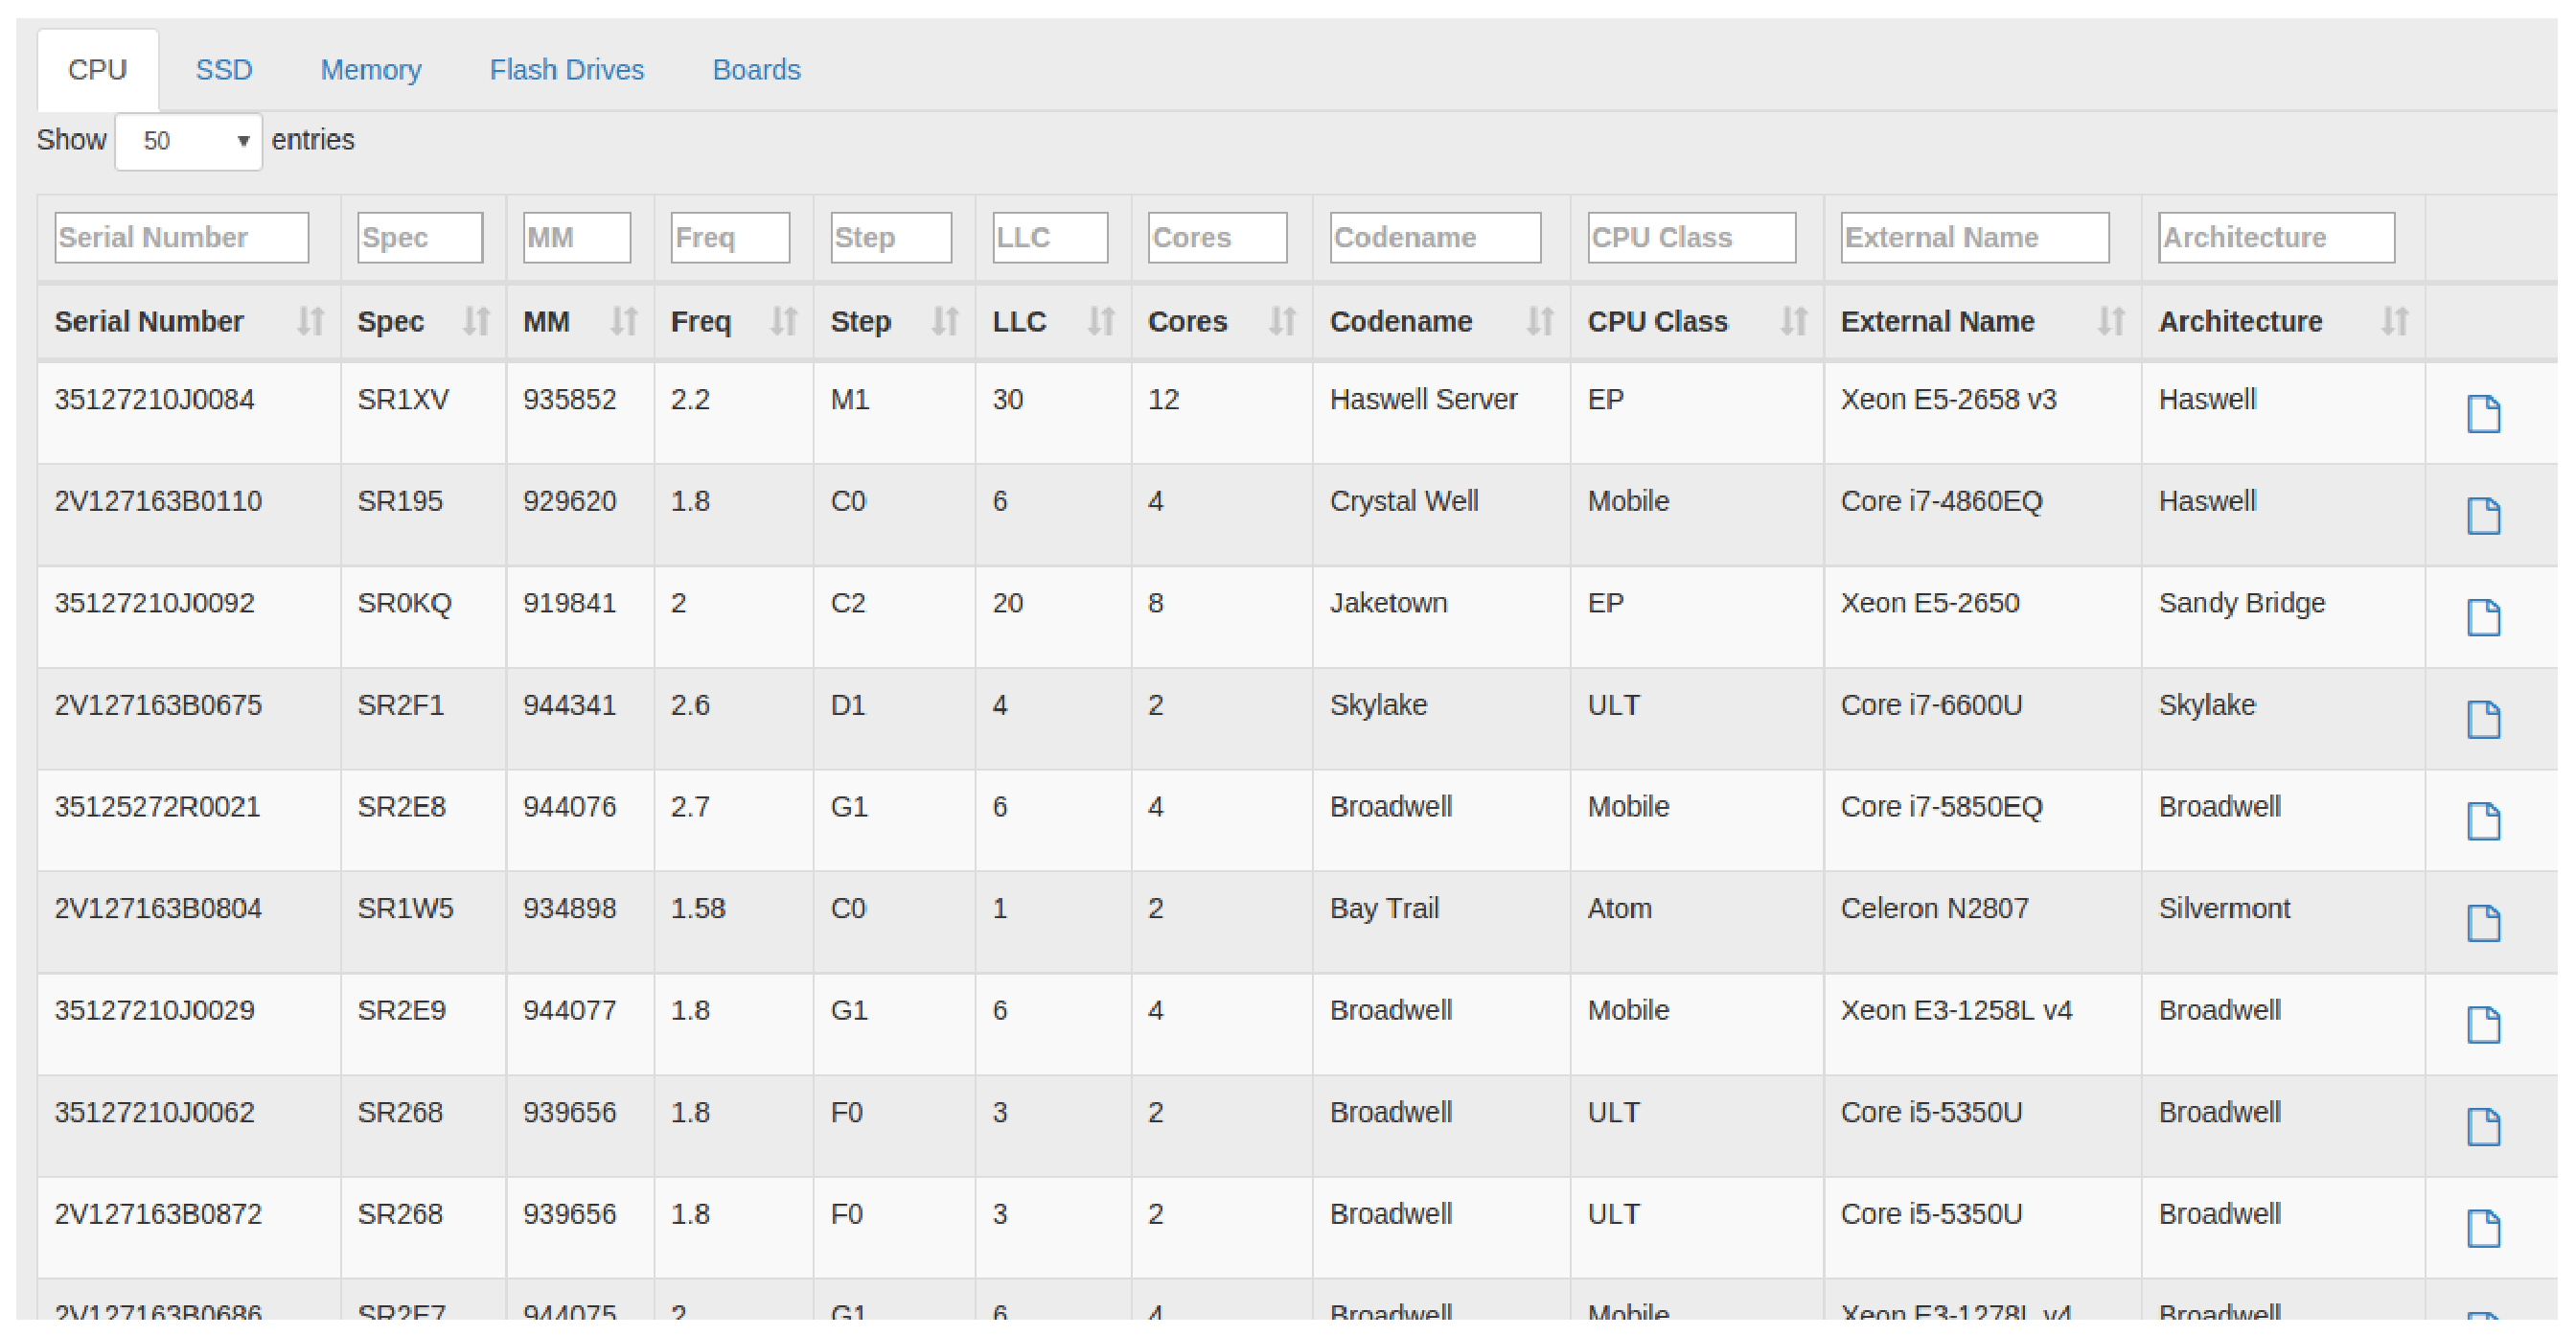
\includegraphics[width=0.9\textwidth]{img-4.eps}
    \caption{The CPU table.}
\end{figure}

\begin{figure}[!ht]
    \centering
    \captionsetup{justification=centering}
    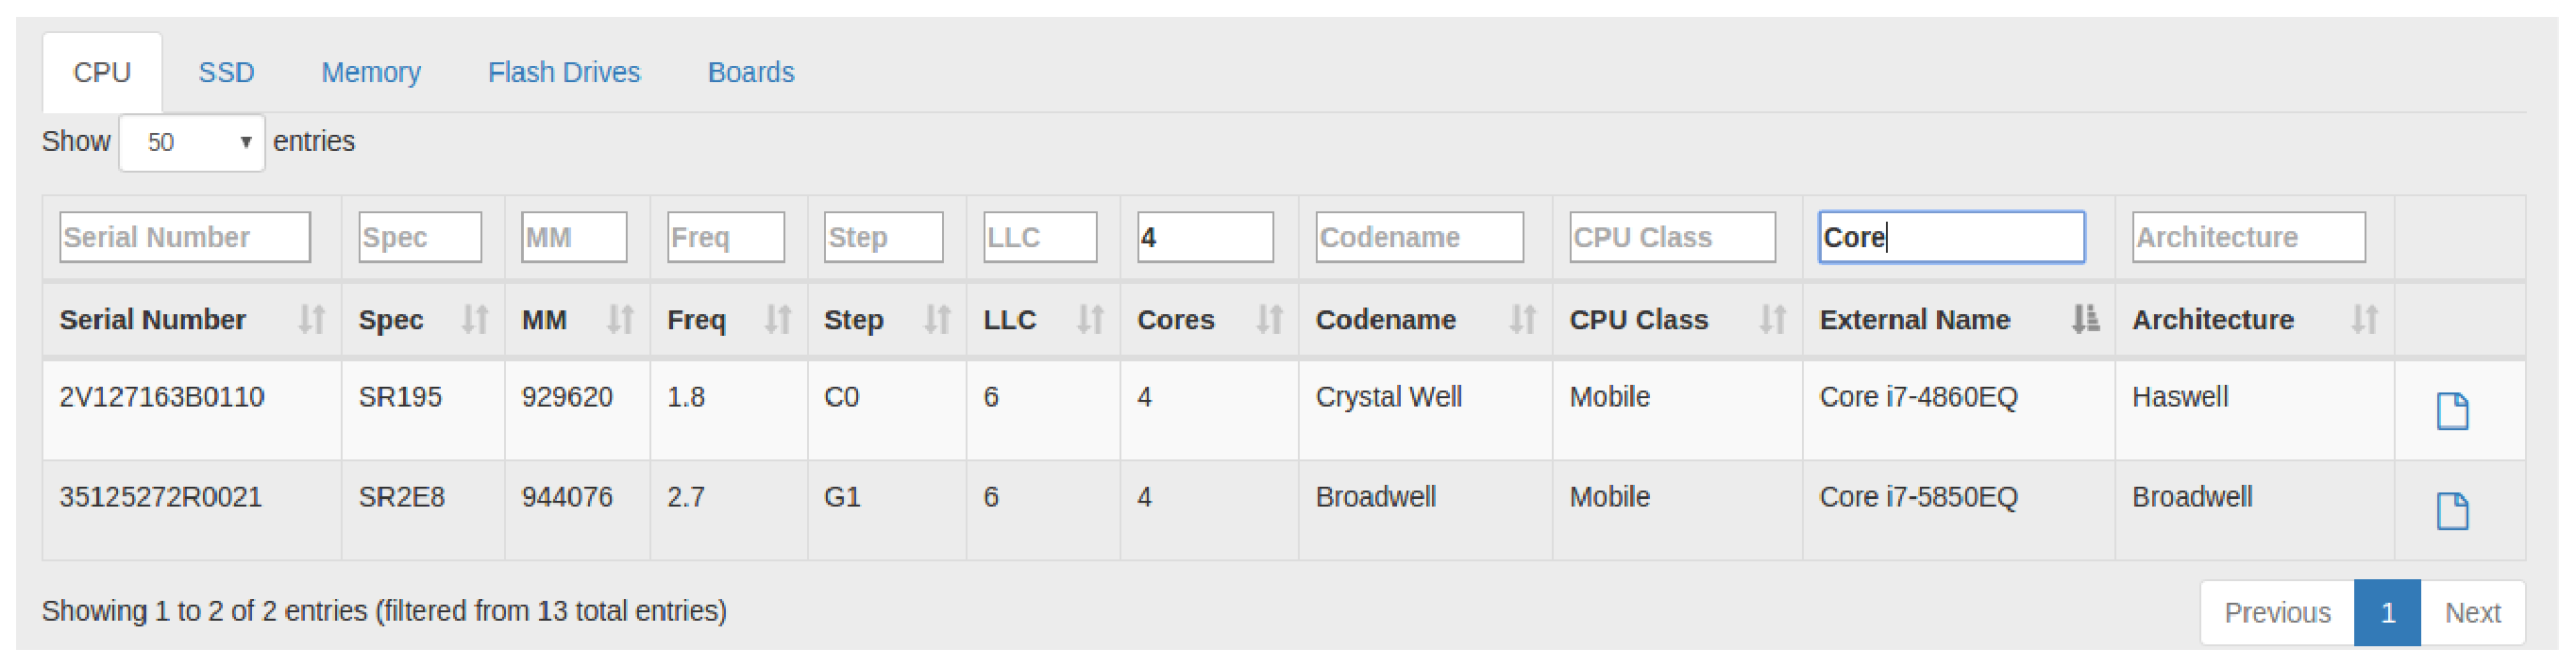
\includegraphics[width=0.9\textwidth]{img-3.eps}
    \caption{Filtering table based on number of cores and external name.}
\end{figure}

\begin{figure}[!ht]
    \centering
    \captionsetup{justification=centering}
    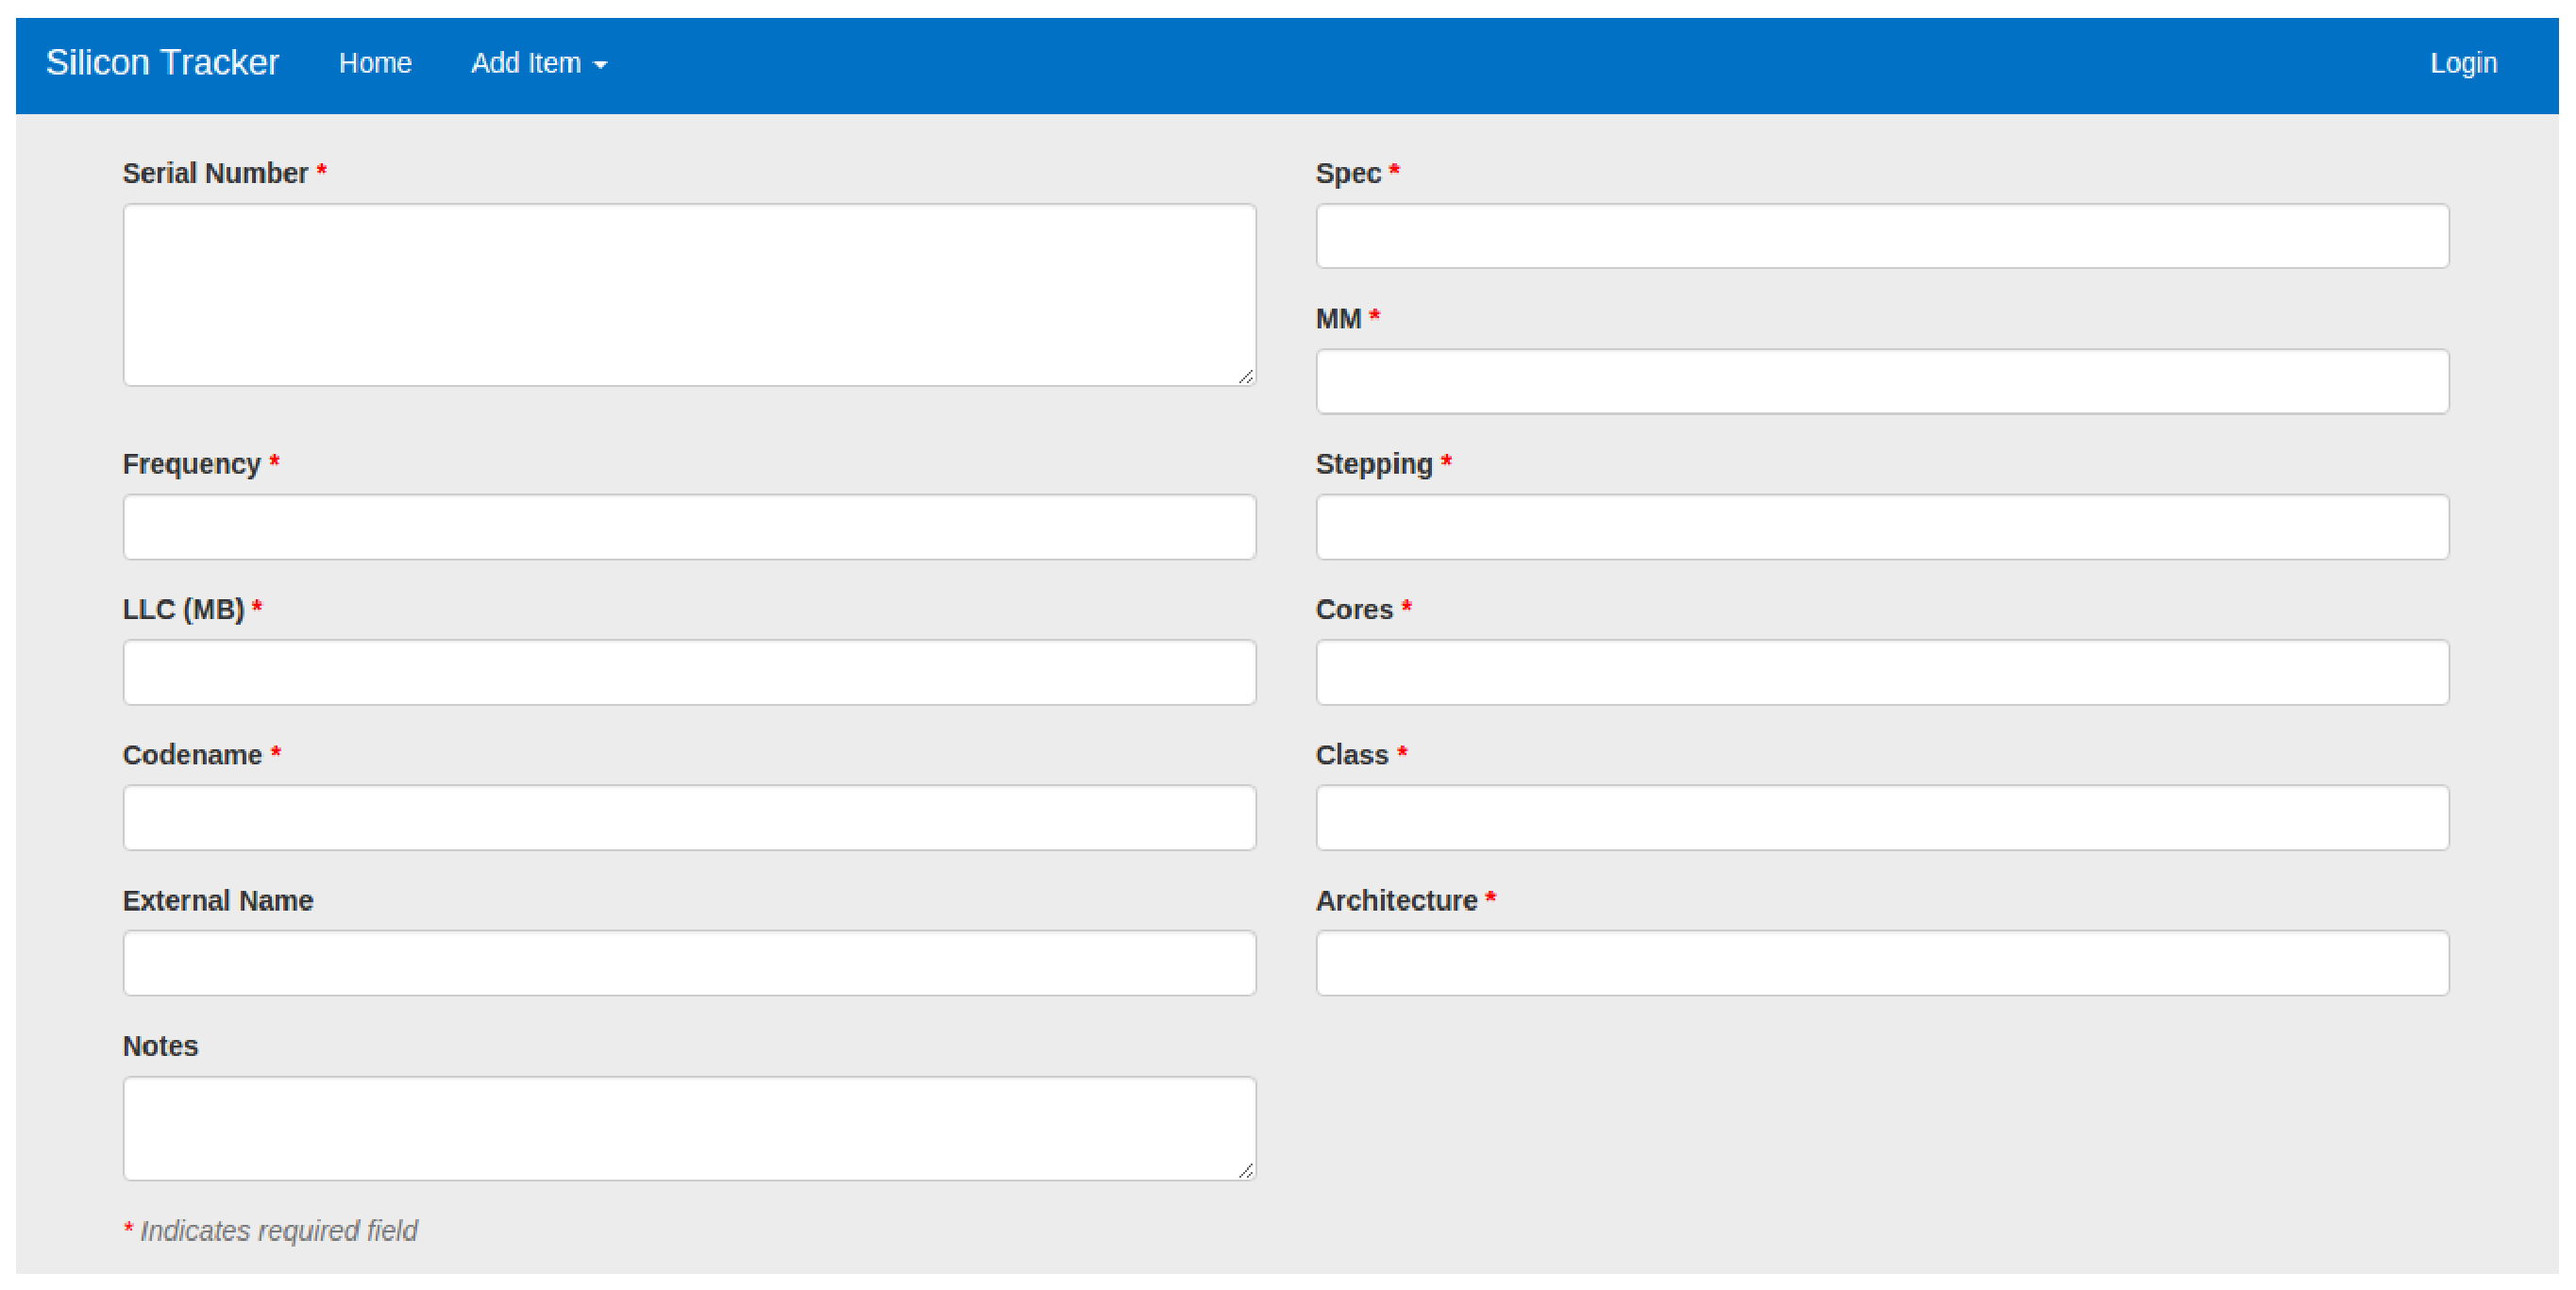
\includegraphics[width=0.9\textwidth]{img-2.eps}
    \caption{The screen for adding a new CPU.}
\end{figure}

\begin{figure}[!ht]
    \centering
    \captionsetup{justification=centering}
    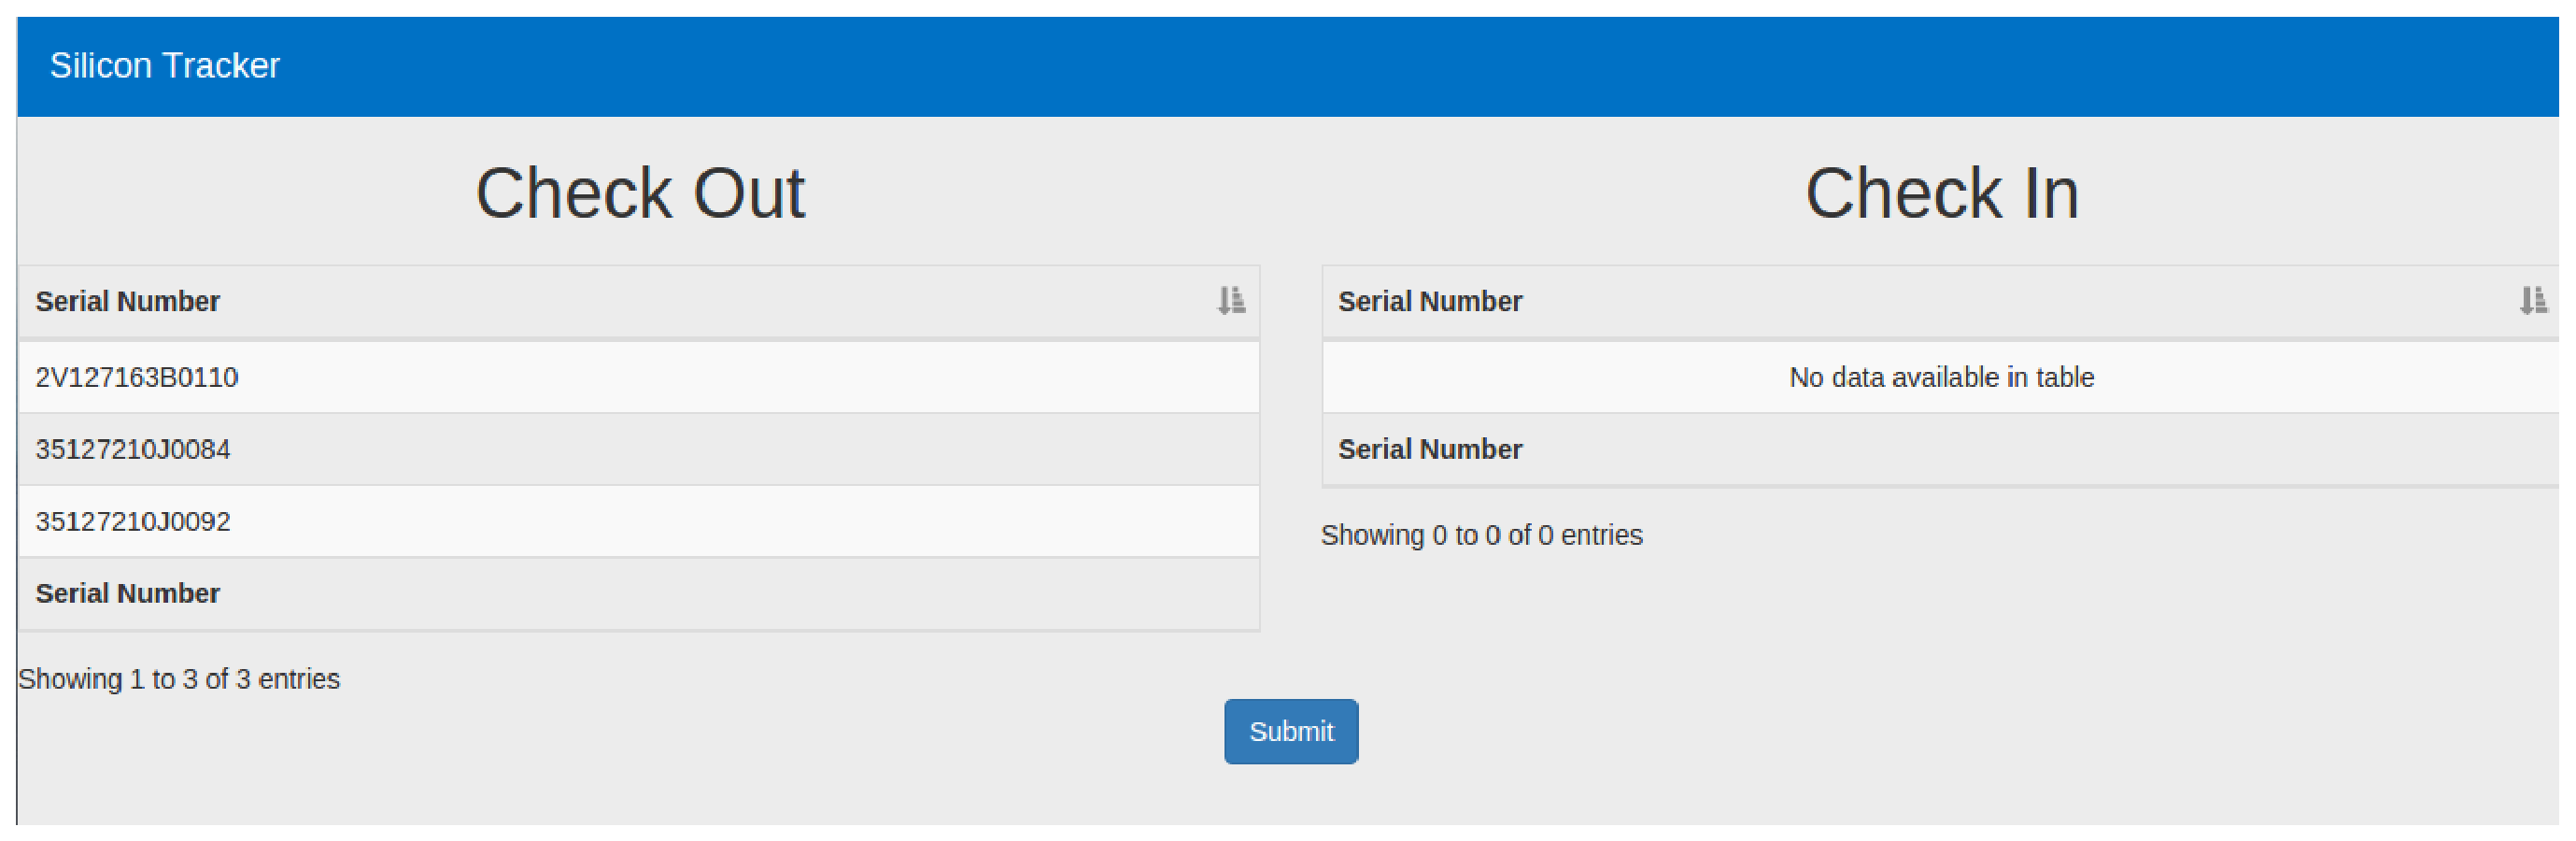
\includegraphics[width=0.9\textwidth]{img-1.eps}
    \caption{The kiosk cart screen, with some items to check out.}
\end{figure}

%\section{Conclusion}
% The conclusion goes here.

\ifCLASSOPTIONcaptionsoff
  \newpage
\fi

% that's all folks
\end{document}